\documentclass[12pt]{article}
\usepackage[margin=1in]{geometry}
\usepackage{amsmath}
\usepackage{amssymb}
\usepackage{fancyhdr}
\usepackage{pgfplots}
\usepackage{graphicx}
\usepackage{enumitem}
\usepackage{hyperref} 
\pgfplotsset{compat=1.16}


\author{Zhijie Xia, Yuan Liu, Zixing Wei, G-69}
\title{CPSC 471 Final Report}


\pagestyle{fancy}
\renewcommand{\headrulewidth}{0pt}
\renewcommand{\footrulewidth}{0pt}


\fancyhf{}
\rhead{
    Final Report
}
\rfoot{
    Page \thepage
}

\begin{document}
\maketitle
\newpage

\textbf{Abstract:}

\vspace*{5mm}
“YourStore” is a non-profit online shopping platform. Aside from its non-profit nature, its functionality is very similar to a retailer’s online shopping website, for example, Best Buy and its bestbuy.ca. It provides small stores a website application that is easy to configure and maintain.
The store owners will be given the permission to list other products, change the inventory, and track all the placed orders. All end users’ data (products, orders, inventories) will be stored in the database that can be accessed and modified when needed. The project’s core concept is providing an opportunity to store owners to sell their
products online, which is realized by a series of core functions, such as customers’ order placement, local stores’ order acceptance and arrange delivery . Order status is also updated at different stages of the order and tracked by all end-users.
Our project has similar functionalities to other commercial online shopping services. It facilitates a complete process of shopping order, realized by many core functions, such as customers’ order placement, sellers’ order acceptance and shipment. Order status is also updated at different stages of the order and tracked by all end-users. All CRUD (create, read, update and delete) functions can be realized via Postman, and our mobile-friendly web app can also visualize the entire user-flow from registration to order complete.
“YourStore” is made with React framework, Redux, Node.js, MongoDB, Express. With Node.js MongoDB, and Express, we were able to develop back-end API in javascript language to implement all necessary CRUD functions, as well as connect our back-end API to a mobile-friendly front-end web app, which is developed with a combination of React, Redux, Bootstrap. All API endpoints are properly connected to our database.


\newpage
\textbf{Introduction:}
\vspace*{5mm}

Since the prolonged pandemic has forced people to increasingly move their works and life online, many small sized
local stores are suffering a plummeting in the number of in store shoppers. Thus, they desire to seize the opportunity to develop online businesses like other large-chain retail stores. This problem is partially solved by online workshops like Amazon, Ebay, and StockX.
Their business model allows business owners to sell other products on their website by charging a substantial percentage of commission. Since the pandemic has lasted for a long time and there is no sign of an end at present, many local small-sized store owners argue the current business model that they build on the online platforms becomes less economically viable and not commercially sustainable for them when a considerable part of their revenue is being taken by the platform provider.

\vspace*{10mm}

\textbf{Our System:}
\vspace*{5mm}

"YourStore" is a non-profit online shopping platform. Aside from its non-profit nature, its functionality is very similar to a retailer’s online shopping website, for example, Best Buy and its bestbuy.ca. It provides small stores a website
application that is easy to configure and maintain. The store owners will be given the permission to list other products, change the inventory, and track all the placed orders. All end users, data (products, orders, inventories) will be stored
in the database that can be accessed and modified when needed. The project’s core concept is providing an opportunity to store owners to sell their products online, which is realized by a series of core functions, such as customers' order placement, local stores'
order acceptance and arrange delivery . Order status is also updated at different stages of the order and tracked by all end-users.

\newpage
\textbf{Project Design Description:}

We have three types of users : \textbf{customer}, \textbf{seller}, and \textbf{administrator}. Each type of user needs to
login first and receive an access token for future interactions with APIs. Note that \textbf{administrator} users
are predefined and an user cannot register himself/herself as a type of \textbf{administrator}.
\vspace*{5mm}

\textbf{Customer:}
After a \textbf{customer} user logs in, he/she would be given a search bar which has a dropdown menu of category and a text input
field.

The customer can choose a particular category from the categories or "All" and search products with the text input. After clicking "Search",
the page would redirect customer to search results, a list of products that meet the searching conditions would be showed on the screen.

The products would be showed with their descriptions, images, prices and inventories information so that the customer can carefully exam.

After the customer decides what products he/she may want, he/she can choose to add the products by clicking "Add To Cart" button, and the product information
would be added into his/her cart.

When the customer decides to checkout, he/she would goes to his/her cart page, and the list of products that the
customer added would show on the screen.

The customer may want to delete some unwantted products by clicking the trashbin icon, thus the product would be
remove from his/her cart.

In order to create orders and actually purchase the products in the cart, the customer must supply a receiver name
and a receiver address to create orders. The receiver name and address would be stored in the database so that the seller can arrange shipping when the order
is paid for.

After creating the products, the customer needs to goto his/her "Orders" page where he/she can find a list of all orders of his/her and do
some actions, for example, "Pay" for the order or "Cancel" the order. While waiting for the products to arrive, the customer can follow the status in his/her
order pages.

\vspace*{5mm}
\textbf{Seller:} After a \textbf{seller} user logs in, he/she would be redirected to a page where he/she can find
all his/her products that are listing in the site for sell.

If there are any products that the seller wants to sell,
he/she can click "Add New Product" buttons, a modal input form would pop up. The seller must fill in the product details
in all blank fields and click "Create Product" to insert the product information in the database so that a customer can find
the product in the search result and potentially add it into the cart and purchase it.

Moreover, when the seller can closely mointor the product information especially the inventory status. The seller would want
to add more inventory when he/she has more products avaiable arrived in stock. Or the product want to increase/decrease price of a
particular product. Maybe he wants to change the description to attract more customers. All the updations can be done in the "My Products" page.

The seller can also see the list of orders that he/she is getting, and the status of the orders(unpaid, paid, unshipped, shipped) to plan the shipment.
Both the seller and the customer of a order would have the same view on the status. When the customer paid for the order, the seller of the
order can now upload shipping label and complete the order.


\vspace*{5mm}
\textbf{Administrator:}

The \textbf{administrator} manages every part of the site, and a administrator user has absolutely full permissions to anything, for example, delete
a user, delete a product, cancel a order.

Thus, the administrator account should be carefully protected and given to trusted ones.




\newpage
\textbf{Project Design EER:}

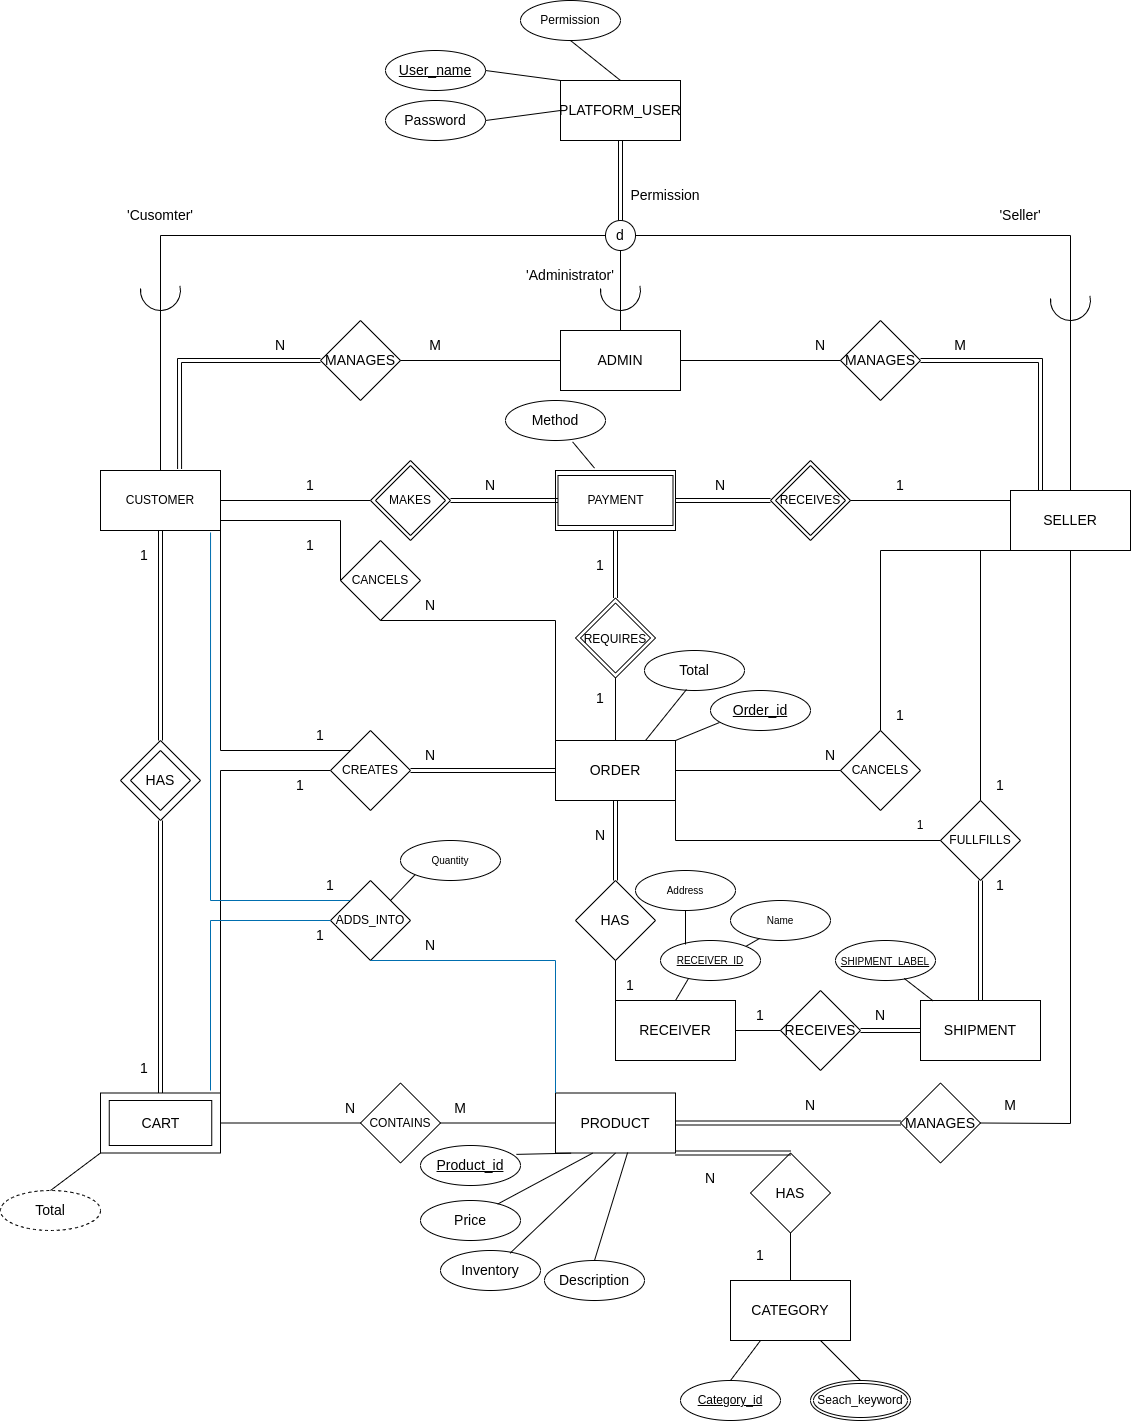
\includegraphics[height=.80\textheight]{Diagrams/onlineShopping_revised.png}

\newpage
\textbf{Implementation RMD:}
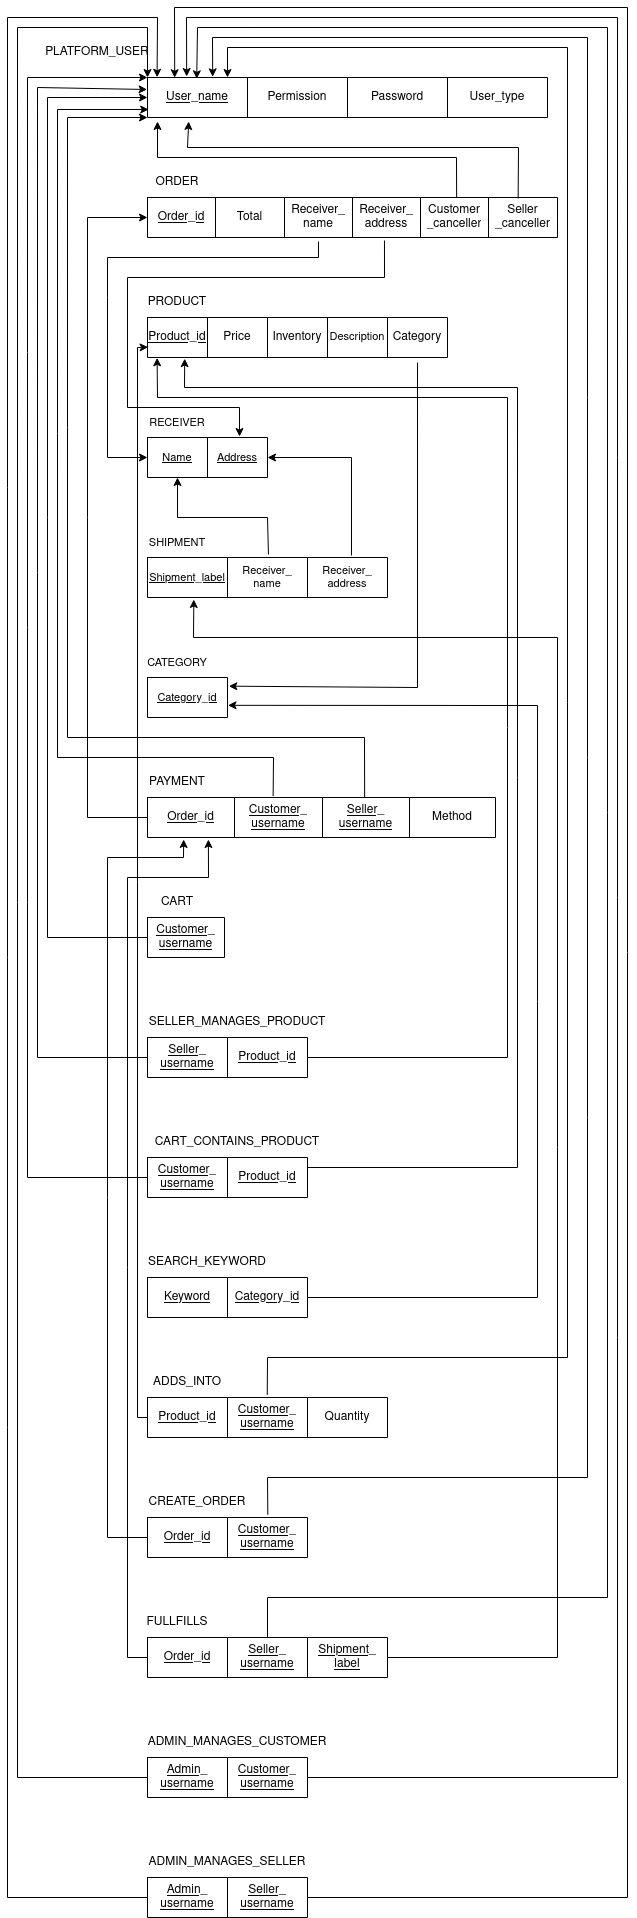
\includegraphics[height=.98\textheight]{Diagrams/relation.png}

\newpage
\textbf{Implementation DBMS:}

We have chosed \textbf{MongoDB} as our DBMS. MongoDB is an open source NoSQL database program
that stores JSON-like documents.

\begin{verbatim}
    Schemas:

    const adminDB = new mongoose.Schema({
        UserName:{
            type:String,
            required:true
        },
        Password:{
            type:String,
            required:true
        },
    })

    const categoryDB = new mongoose.Schema({
        Title:{
            type:String,
            required:true
        },
        Products:[String]
    })

    const customerSchema = new mongoose.Schema({
        UserName:{
            type:String,
            required:true
        },
        Password:{
            type:String,
            required:true
        },
        Cart:{
            type:[String],
            required:true
        },
        Orders:{
            type:[String],
            required:true
        },
    })


    const orderDB = new mongoose.Schema({
        CustomerID:{
            type:String,
            required:true
        },
        SellerID:{
            type:String,
            required:true
        },
        Total:{
            type:Number,
            required:true
        },
        ReceiverName:{
            type:String,
            required:true
        },
        ReceiverAddress:{
            type:String,
            required:true
        },
        Payment:{
            type:Boolean,
            required:true,
        },
        Cancelled:{
            type:Boolean,
            required:true
        },
        Shipped:{
            type:Boolean,
            required:true
        },
        ShipmentLabel:{
            type:String,
            required:true
        },
        Product:{
            type:String,
            required:true
        }
    })


    const productDB = new mongoose.Schema({
        SellerID:{
            type:String,
            required:true
        },
        Title:{
            type:String,
            required:true
        },
        Price:{
            type:Number,
            required:true
        },
        Inventory:{
            type: Number,
            required:true
        },
        Description:{
            type:String,
            required:true
        },
        SearchKeys:{
            
        required:true
        },
        Category:{
            type: String,
            required:true
        },
        Owned:{
            type: Boolean,
            required:true
        }
    })


    const sellerDB = new mongoose.Schema({
        UserName: {
            type: String,
            required: true
        },
        Password: {
            type: String,
            required: true
        },
        CardNumber: {
            type: String,
            required: true
        },
        Orders: {
            type: [String],
            required: true
        },
        Products: {
            type: [String],
            required: true
        },
    })



    // find all products that are not being deleted
    let allProducts = await productDB.find();
    allProducts = allProducts.filter((product)=>{
    return product.Owned;
    });


    // create new category
    const newCategory = new categoryDB(
    {               // parse JSON
            Title: req.body.Title
        })
    await newCategory.save();


    // find all orders information with derived order status
    actualOrders = await orderDB.find();
    let orderInfo;
    orderInfo = await Promise.all(actualOrders.map(async (order) => {
    let product = await productDB.findOne({ "_id": order.Product });
    let status;
    if (!order.Payment) {
            status = "Unpaid"
        }
    else {
            if (order.Shipped) {
                    status = "Shipped"
                }
            else {
                    status = "Unshipped"
                }
        }
    if (order.Cancelled) {
            status = "Cancelled";
        }
    return {
            "Order":order,
            "Product":product,
            "Status":status
        }
    }));

    // find the list of all categories
    const allCategories = await categoryDB.find()

    // delete a category
    await res.categoryInstance.remove()

    // find a particular category
    categoryInstance = await categoryDB.findOne({ "Title": req.params.id })


    // find the list of all orders of a particular customer
    const customerOrderIDs = res.customerInstance.Orders;
    let actualOrders;
    actualOrders = await Promise.all(customerOrderIDs.map(async (orderID) => {
    return orderDB.findOne({ "_id": orderID });
    }));
    let orderInfo;
    orderInfo = await Promise.all(actualOrders.map(async (order) => {
    let product = await productDB.findOne({ "_id": order.Product });
    let status;
    if (!order.Payment) {
            status = "Unpaid"
        }
    else {
            if (order.Shipped) {
                    status = "Shipped"
                }
            else {
                    status = "Unshipped"
                }
        }
    if (order.Cancelled) {
            status = "Cancelled";
        }
    return {
            "OrderNumber": order._id,
            "SellerID": order.SellerID,
            "ProductName": product.Title,
            "Price": order.Total,
            "ReceiverName": order.ReceiverName,
            "ReceiverAddress": order.ReceiverAddress,
            "Status": status,
            "ShipmentLabel": order.ShipmentLabel
        }
    }));


    // find the cart details of a customer
    const cart = res.customerInstance.Cart;

    let total = 0;

    let products = await Promise.all(cart.map(async (productID) => {
    const product = await productDB.findOne({ "_id": productID });
        return product;
    }));


    // add a product into the customer's cart
    res.customerInstance.Cart.push(req.body.ProductID);
    await res.customerInstance.save()


    // delete a product from the customer's cart 
    var index = res.customerInstance.Cart.indexOf(req.body.ProductID);
    if (index != -1) {
        res.customerInstance.Cart.splice(index, 1);
    }
    await res.customerInstance.save();


    // delete all the orders of a customer 
    res.customerInstance.Orders = []
    await res.customerInstance.save();



    // create orders with respect to the customer's cart 
    for (const product of req.body.Products) {

        let productInstance;
        productInstance = await productDB.findOne({ "_id": product._id });
        if (productInstance.Inventory > 0) {

            productInstance.Inventory = productInstance.Inventory - 1;
            await productInstance.save();
        }
        else {
            outOfStock = true;
            continue;
        }

        let newOrder = new orderDB(
            {
                CustomerID: req.params.id,
                SellerID: product.SellerID,
                Total: product.Price,
                ReceiverName: req.body.ReceiverName,
                ReceiverAddress: req.body.ReceiverAddress,
                Payment: false,
                Cancelled: false,
                Shipped: false,
                ShipmentLabel: "None",
                Product: product._id
            });

        await newOrder.save();

        res.customerInstance.Orders.push(newOrder._id);
        await res.customerInstance.save();

        let sellerInstance;
        sellerInstance = await sellerDB.findOne({ "UserName": product.SellerID })
        sellerInstance.Orders.push(newOrder._id)
        await sellerInstance.save();

    }
    res.customerInstance.Cart = [];
    await res.customerInstance.save();
    


    // create a new customer 
    const newcustomer = new customerDB(
    {  
        UserName: req.body.UserName,
        Password: req.body.Password,
        Cart: []
    })
    const salt = await bcrypt.genSalt(10);
    newcustomer.Password = await bcrypt.hash(newcustomer.Password, salt);
    await newcustomer.save()


    // get a particular customer's detail
    customerInstance = await customerDB.findOne({ UserName: req.params.id })



    // arrange shipment for an order 
    res.orderInstance.Shipped = true;
    res.orderInstance.ShipmentLabel = req.body.ShippingLabel;
    await res.orderInstance.save();


    // get the list of all orders 
    const allOrders = await orderDB.find();


    // create a new order 
    const newOrder = new orderDB(
        {
            CustomerID: req.body.CustomerID,
            SellerID: req.body.SellerID,
            Total: req.body.Total,
            ReceiverName: req.body.ReceiverName,
            ReceiverAddress: req.body.ReceiverAddress,
            Payment: false,
            Cancelled: false,
            Shipped: false,
            ShipmentLabel: "None",
            Product: req.body.Product
        })
    const savedOrder = await newOrder.save()


    // delete a particular order 
    await res.orderInstance.remove()

    // remove all orders 
    await orderDB.remove({});

    // get a particular order instance 
    orderInstance = await orderDB.findOne({ "_id": req.params.id })


    // get a list of products with category info
    allProducts = await categoryDB.findOne({ "Title": category });
    allProducts = allProducts.Products;
    allProducts = await Promise.all(allProducts.map(async (productID) => {
        const product = await productDB.findOne({ "_id": productID });
        return product;
    }));



    // get a list of products with searchKey 
    allProducts = await categoryDB.find();
    allProducts = allProducts.filter((product) => {
                return (product.Title == searchKey || product.SearchKeys.includes(searchKey));
    });


    // create a product
    const newProduct = new productDB(
    {
        SellerID: req.body.SellerID,
        Title: req.body.Title,
        Price: req.body.Price,
        Inventory: req.body.Inventory,
        Description: req.body.Description,
        SearchKeys: req.body.SearchKeys,
        Category: req.body.Category,
        Owned: true,
    })

    const savedproduct = await newProduct.save()

    belongingCategory = await categoryDB.findOne({ "Title": req.body.Category });
    belongingCategory.Products.push(savedproduct._id);
    await belongingCategory.save();

    let belongingSeller = await sellerDB.findOne({ "UserName": req.body.SellerID });
    belongingSeller.Products.push(savedproduct._id);
    await belongingSeller.save();


    // update a product 
    if (req.body.Title) {
        res.productInstance.Title = req.body.Title
    }
    if (req.body.Price) {
        res.productInstance.Price = req.body.Price
    }
    if (req.body.Description) {
        res.productInstance.Description = req.body.Description
    }
    if (req.body.Category) {
        res.productInstance.Category = req.body.Category
    }
    if (req.body.SearchKeys) {
        res.productInstance.SearchKeys = req.body.SearchKeys
    }
    if (req.body.Inventory) {
        res.productInstance.Inventory = req.body.Inventory
    }
    const updatedProduct = await res.productInstance.save()


    // delete a product 
    const sellerInstance = await sellerDB.findOne({ "UserName": res.productInstance.SellerID });

    let index = sellerInstance.Products.indexOf(res.productInstance._id);
    if (index > -1) {
        sellerInstance.Products.splice(index, 1); // 2nd parameter means remove one item only
    }

    await sellerInstance.save();

    res.productInstance.Owned = false;
    await res.productInstance.save();

    let categoryInstance = await categoryDB.findOne({ "Title": res.productInstance.Category })
    index = categoryInstance.Products.indexOf(res.productInstance._id);
    if (index > -1) {
        categoryInstance.Products.splice(index, 1); // 2nd parameter means remove one item only
    }
    await categoryInstance.save();


    // get a particular product 
    productInstance = await productDB.findOne({ "_id": req.params.id })



    // get the list of all orders of a seller
    const sellerOrderIDs = res.sellerInstance.Orders;
    let actualOrders;
    actualOrders = await Promise.all(sellerOrderIDs.map(async (orderID) => {
        return orderDB.findOne({ "_id": orderID });
    }));
    let orderInfo;
    orderInfo = await Promise.all(actualOrders.map(async (order) => {
        let product = await productDB.findOne({ "_id": order.Product });
        let status;
        if (!order.Payment) {
            status = "Unpaid"
        }
        else {
            if (order.Shipped) {
                status = "Shipped"
            }
            else {
                status = "Unshipped"
            }
        }
        if (order.Cancelled) {
            status = "Cancelled";
        }
        return {
            "OrderNumber": order._id,
            "CustomerID": order.CustomerID,
            "ProductName": product.Title,
            "Price": order.Total,
            "ReceiverName": order.ReceiverName,
            "ReceiverAddress": order.ReceiverAddress,
            "Status": status,
            "ShipmentLabel": order.ShipmentLabel
        }
    }));


    // get the a particular order of a particular seller 
    const productIDs = res.sellerInstance.Products;
    let allProducts = await Promise.all(productIDs.map(async (productID) => {
        let productInstance = await productDB.findOne({ "_id": productID });
        return {
            "ProductNumber": productInstance._id,
            "ProductTitle": productInstance.Title,
            "Inventory": productInstance.Inventory,
            "Description": productInstance.Description,
            "Price": productInstance.Price
        }
    }));


    // create a new seller 
    const newSeller = new sellerDB(
        {
            UserName: req.body.UserName,
            Password: req.body.Password,
            Orders: [],
            Products: []
        })

    const salt = await bcrypt.genSalt(10);
    newSeller.Password = await bcrypt.hash(newSeller.Password, salt);
    await newSeller.save()


    // delete a seller 
    await res.sellerInstance.remove()


    // delete a particular seller's orders 
    res.sellerInstance.Orders = []
    await res.sellerInstance.save();


    // get a particular seller instance
    sellerInstance = await sellerDB.findOne({ UserName: req.params.id })
\end{verbatim}













\newpage

\textbf{Postman Docuementation:}

\begin{center}
    https://documenter.getpostman.com/view/20517678/Uyr4LftC
\end{center}

\newpage
\textbf{User Guide:}

\vspace*{5mm}
\textbf{1: Sign in as admin}

Fill in user name as “SuperUser” and password “sodu”. Then click “Login”.

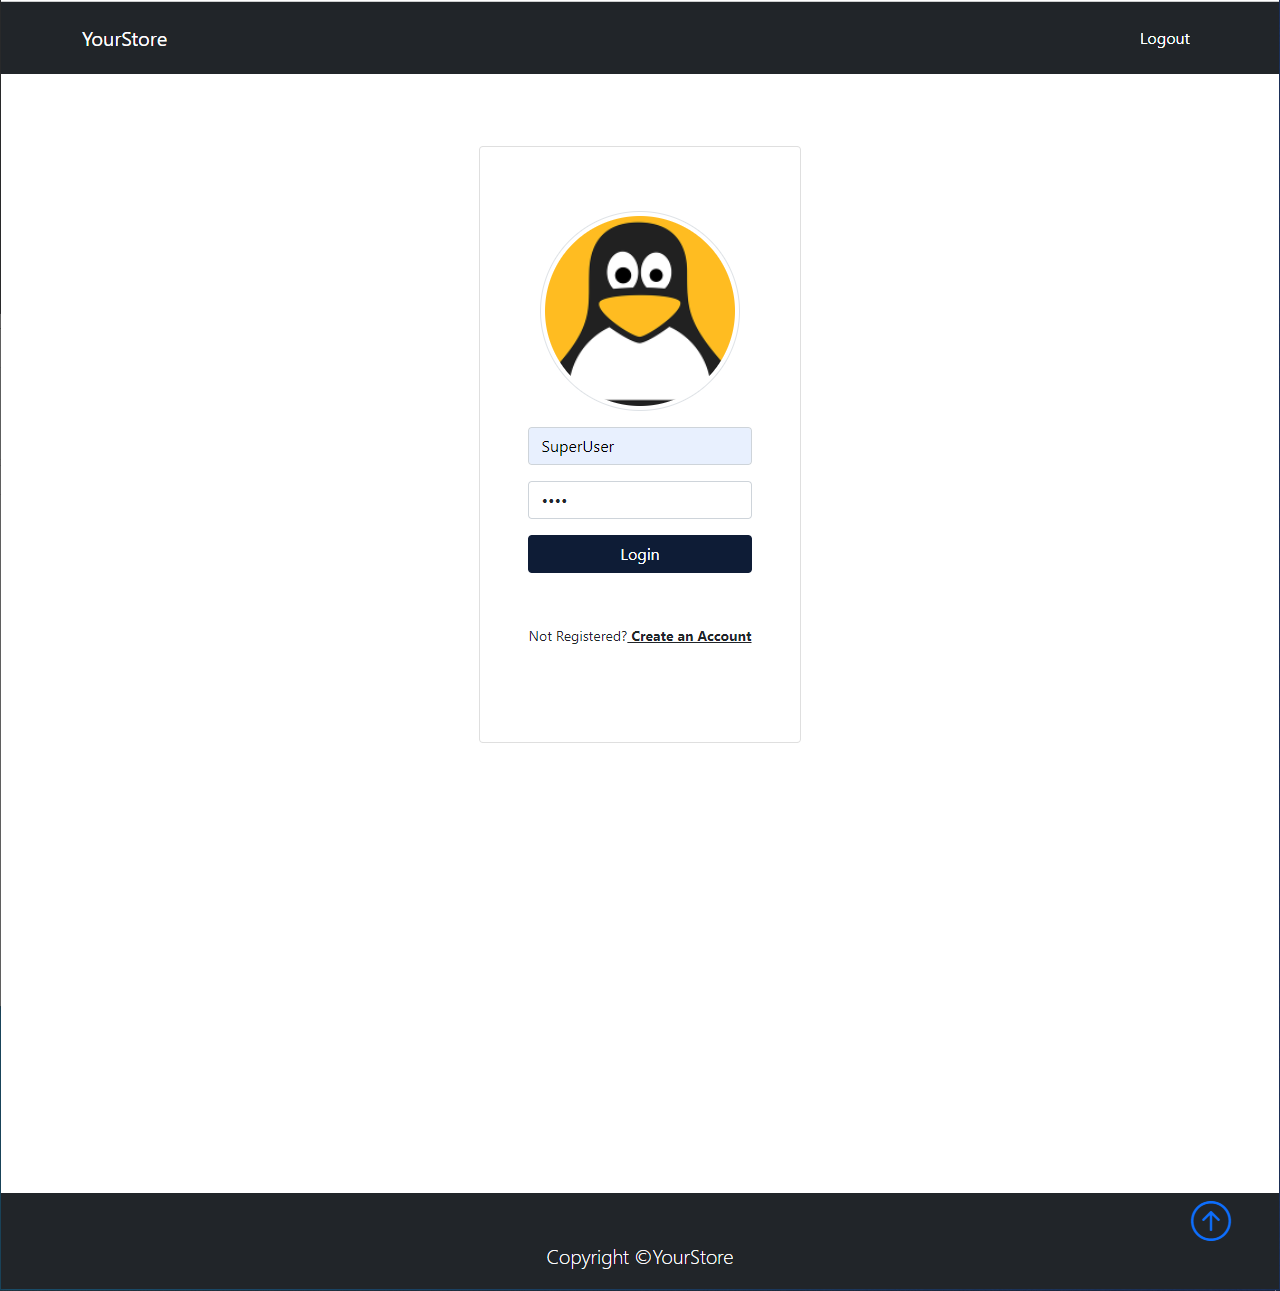
\includegraphics[width=0.45\textwidth]{UserGuideImage/1.png}
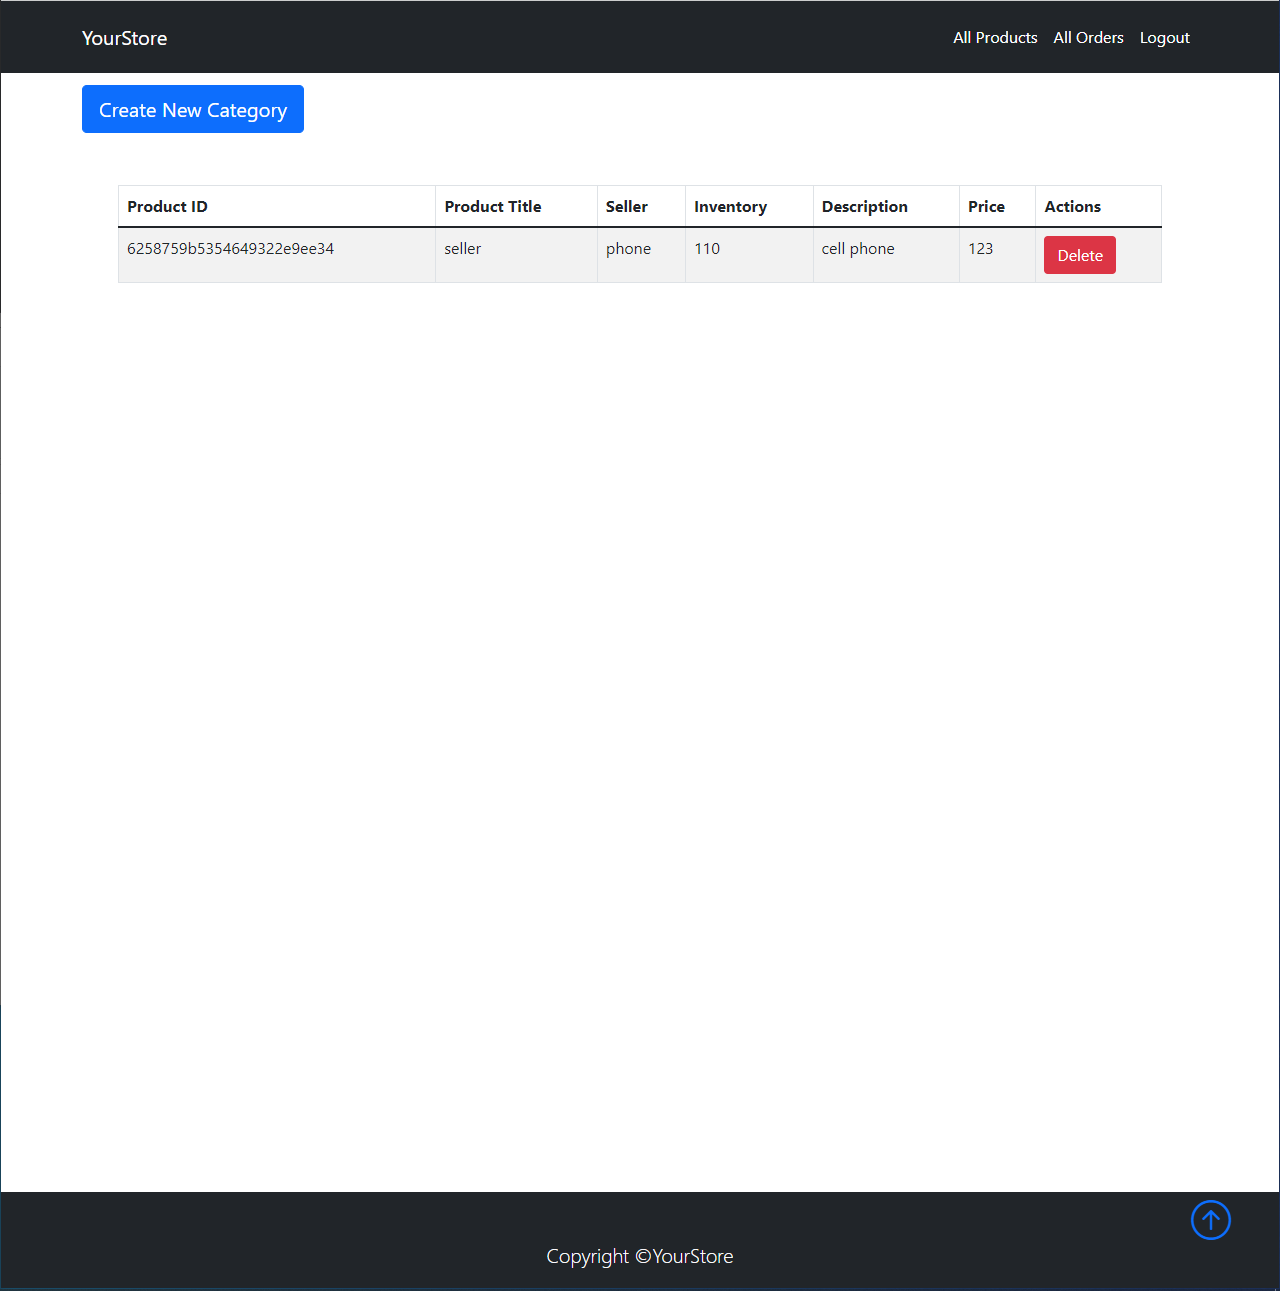
\includegraphics[width=0.45\textwidth]{UserGuideImage/2.png}

\vspace*{5mm}
\textbf{2: Admin manage products}

\hspace*{5mm}\textbf{2.1: Create a new category}

You can access “All Products” page by automatically sign in as admin or click “All Products”
at nav bar. In “All Products” page, admin can create a new category as below.

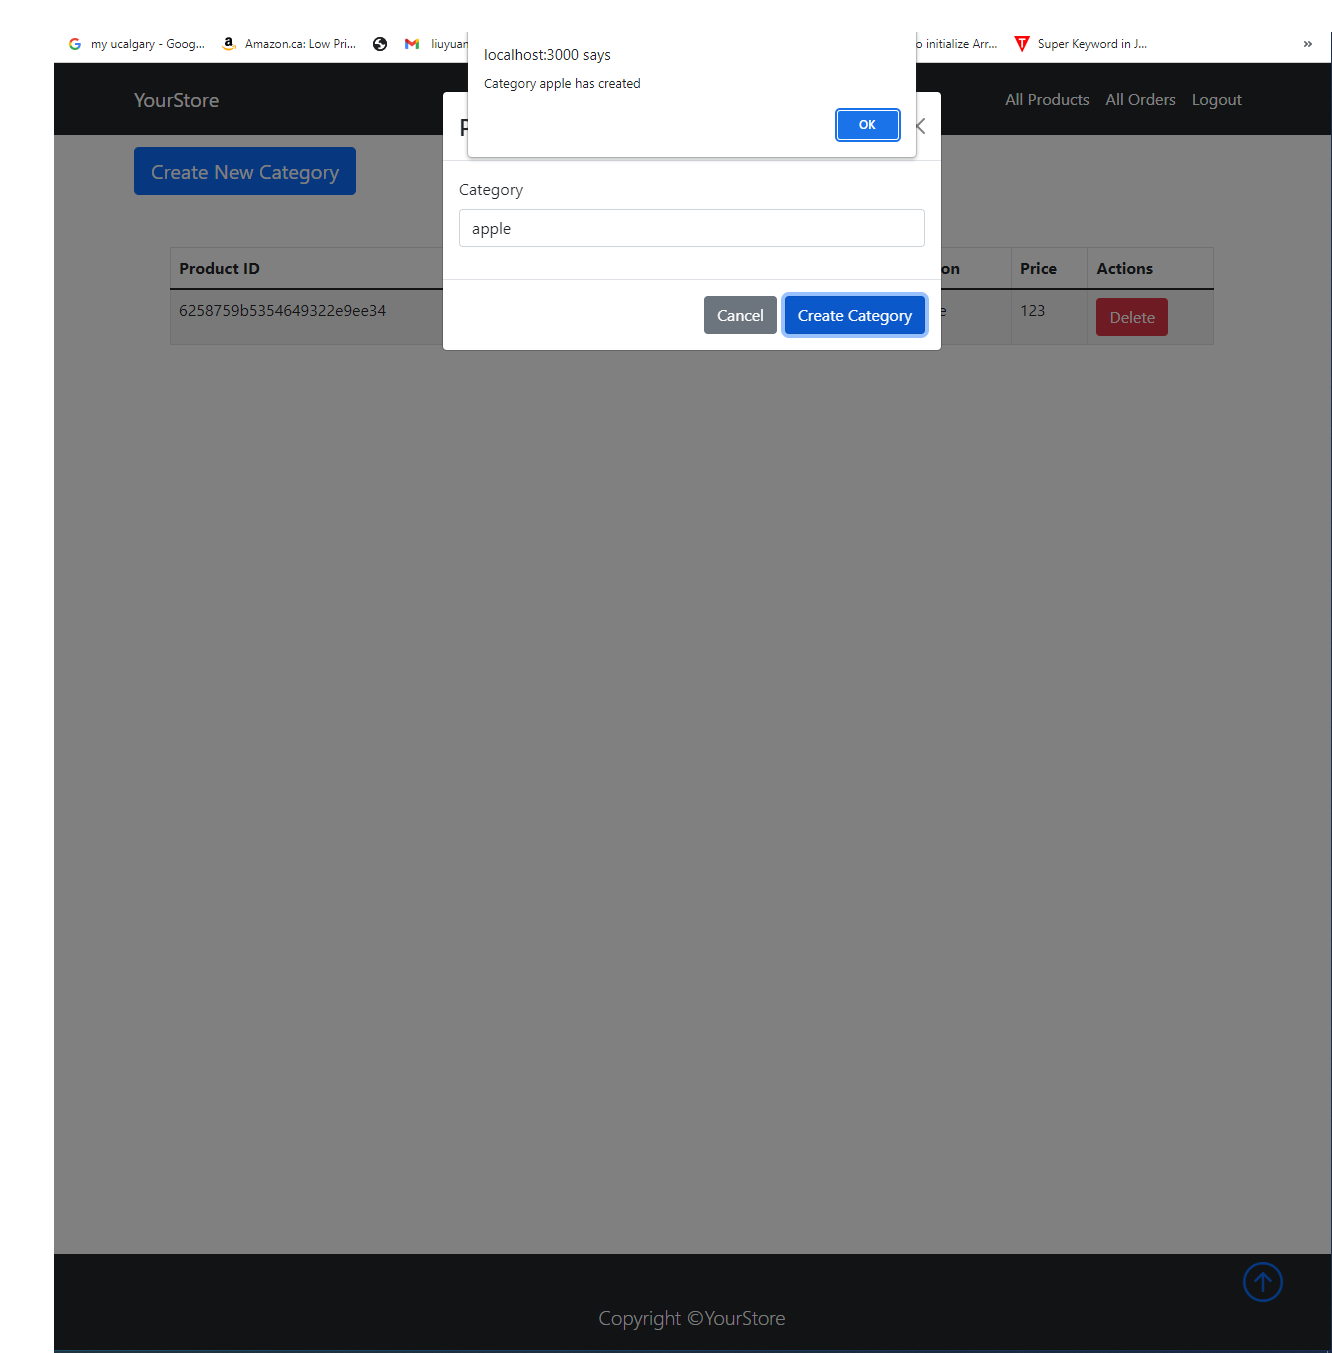
\includegraphics[width=0.45\textwidth]{UserGuideImage/3.png}

\newpage
\hspace*{5mm}\textbf{2.2: Delete products}

In “All Products” page, admin can delete any existing products as below.

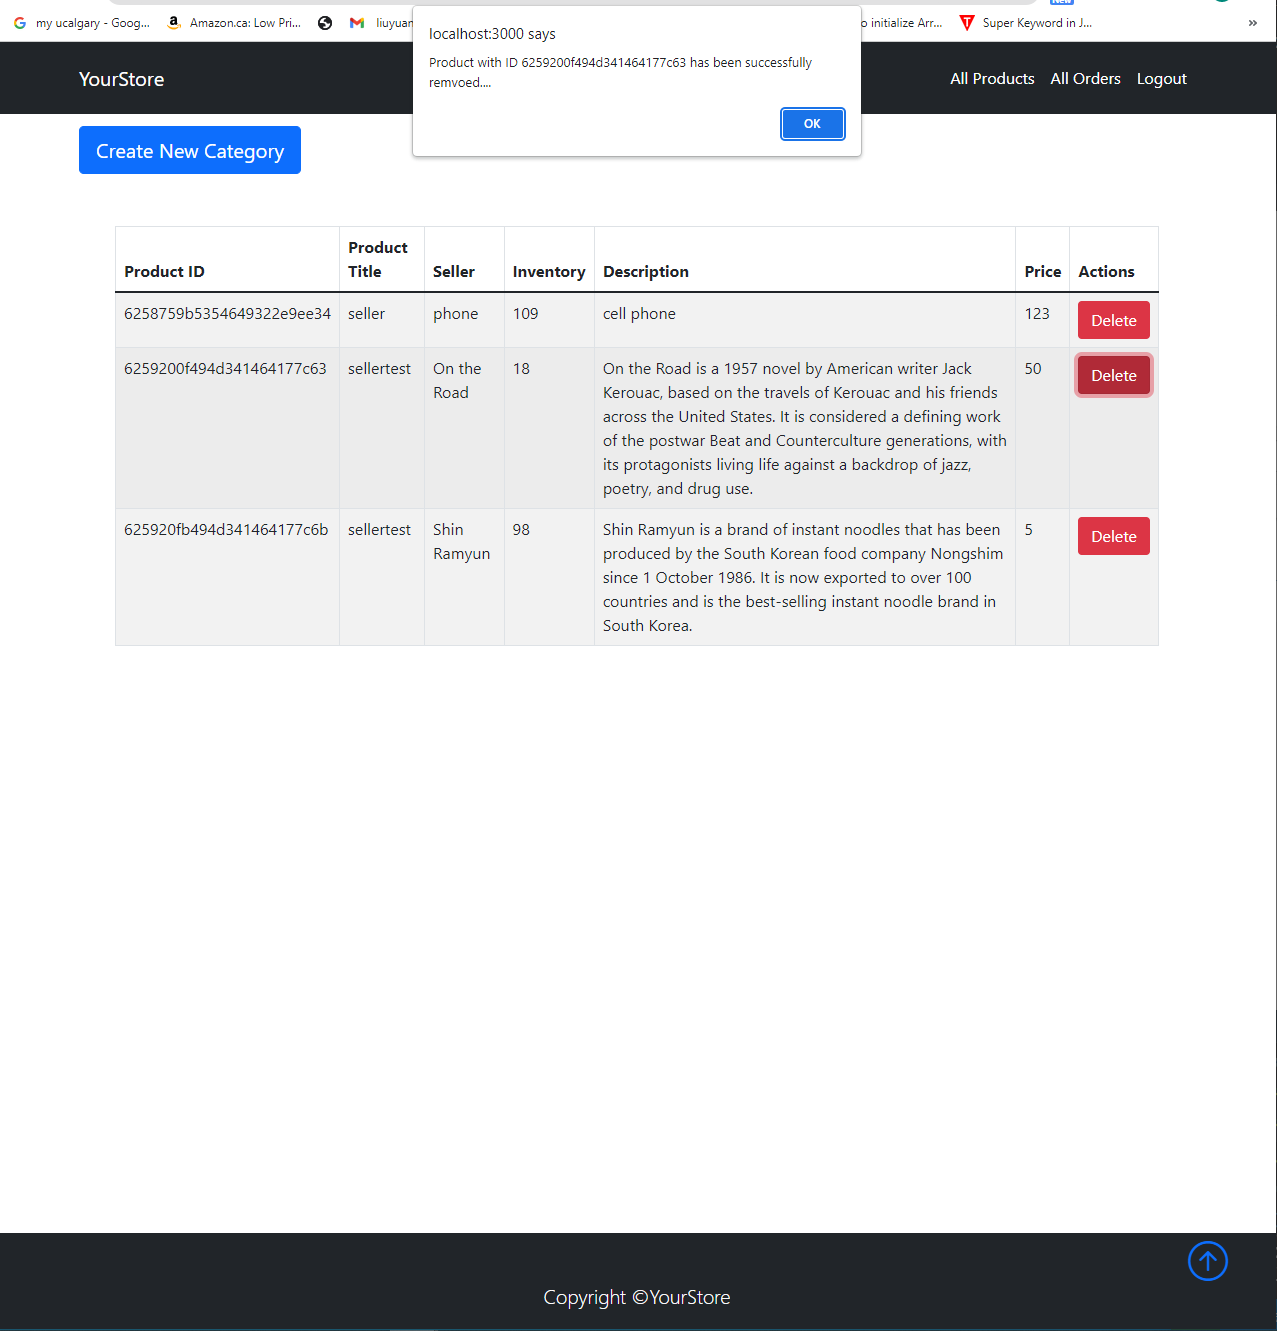
\includegraphics[width=0.45\textwidth]{UserGuideImage/4.png}

\vspace*{5mm}
\textbf{3: Admin manage orders}

Click “All Orders” on nav bar, admin can delete any existing orders as below.

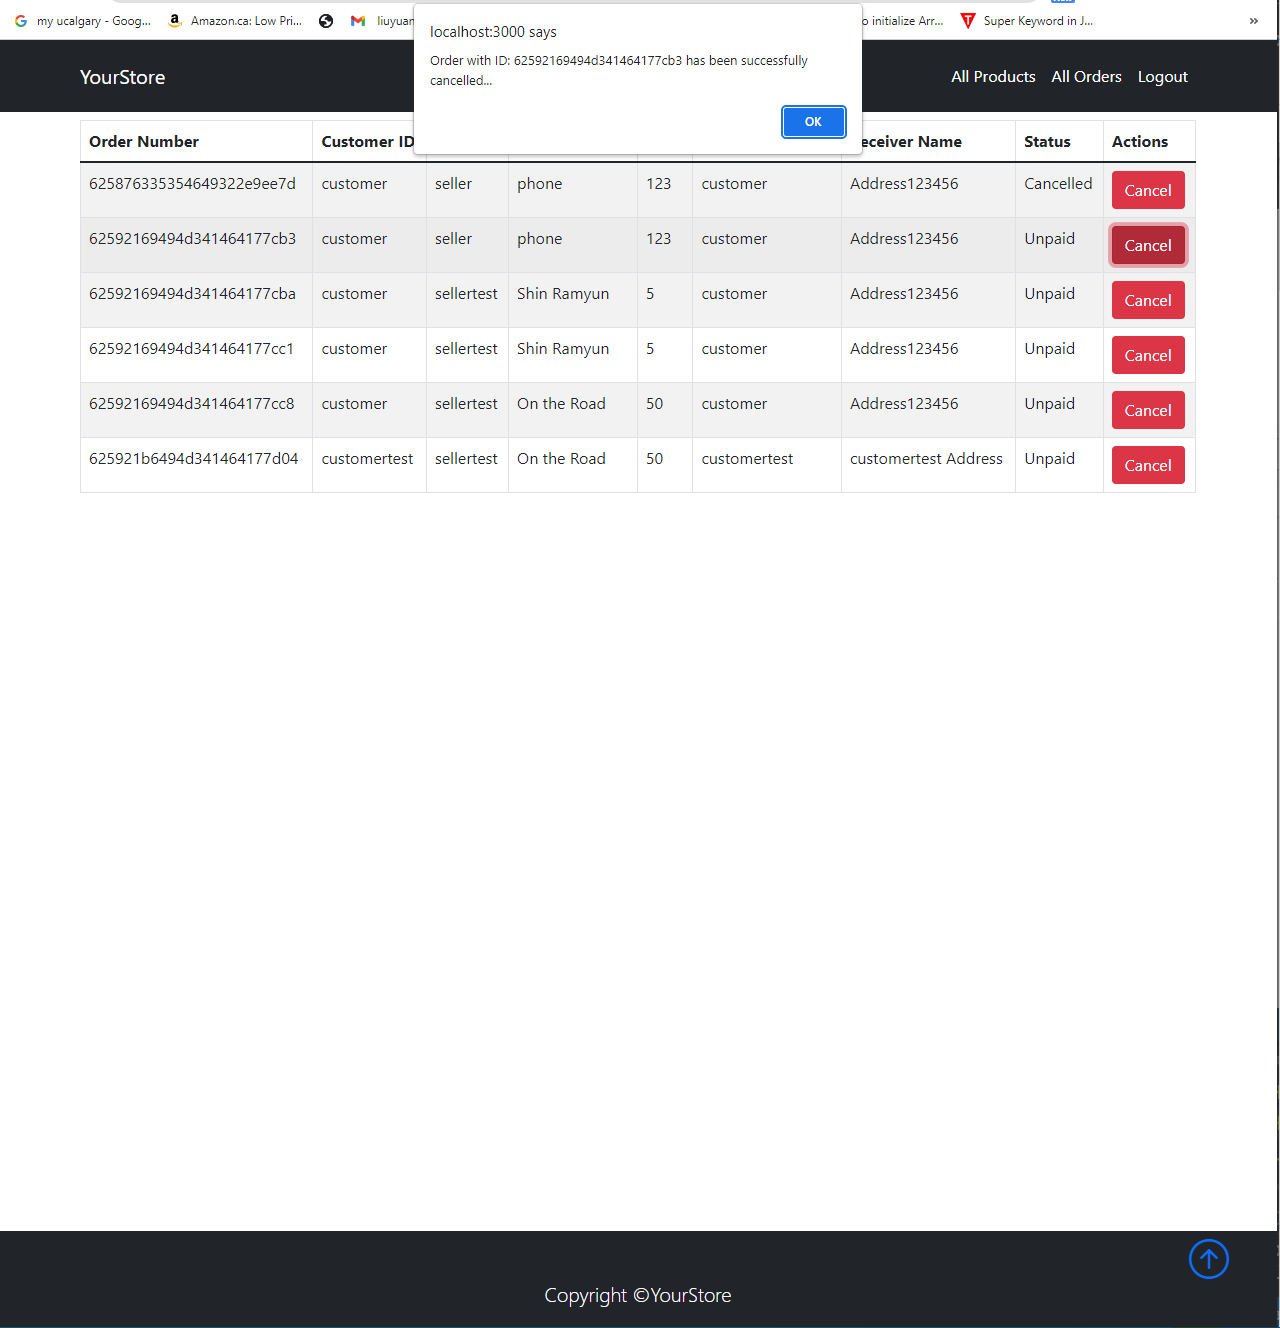
\includegraphics[width=0.45\textwidth]{UserGuideImage/5.png}

\newpage
\textbf{4: Sign in as seller}

Register a seller account and then sign in with the information that used for account registration.

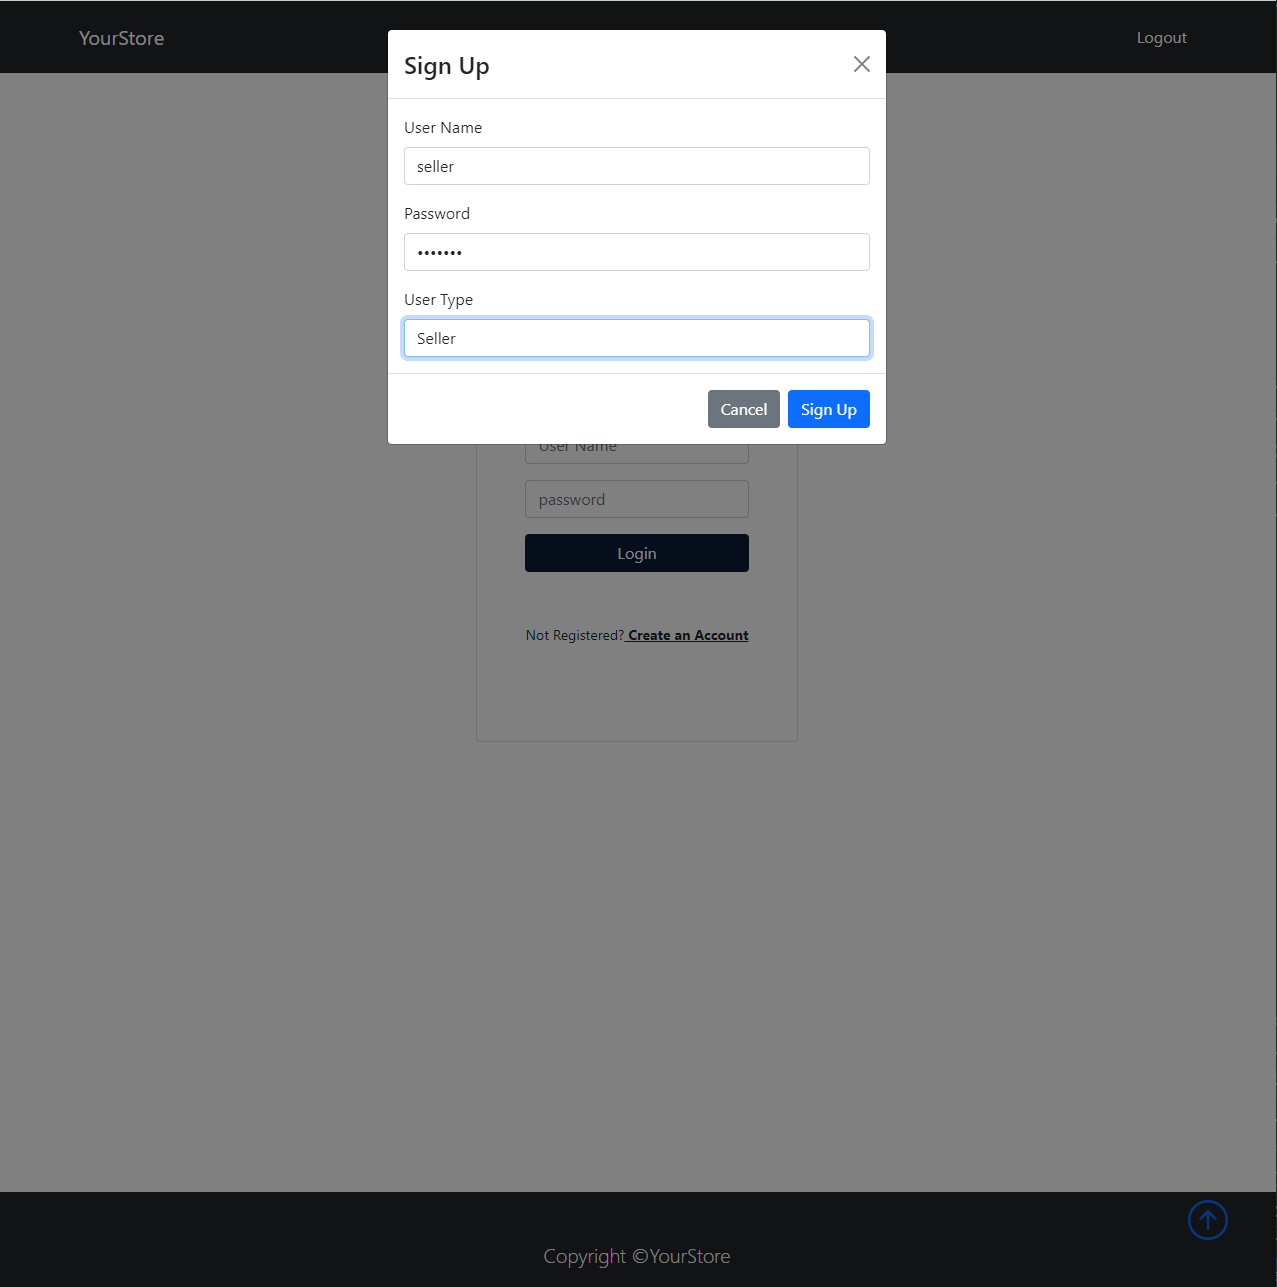
\includegraphics[width=0.45\textwidth]{UserGuideImage/6.png}
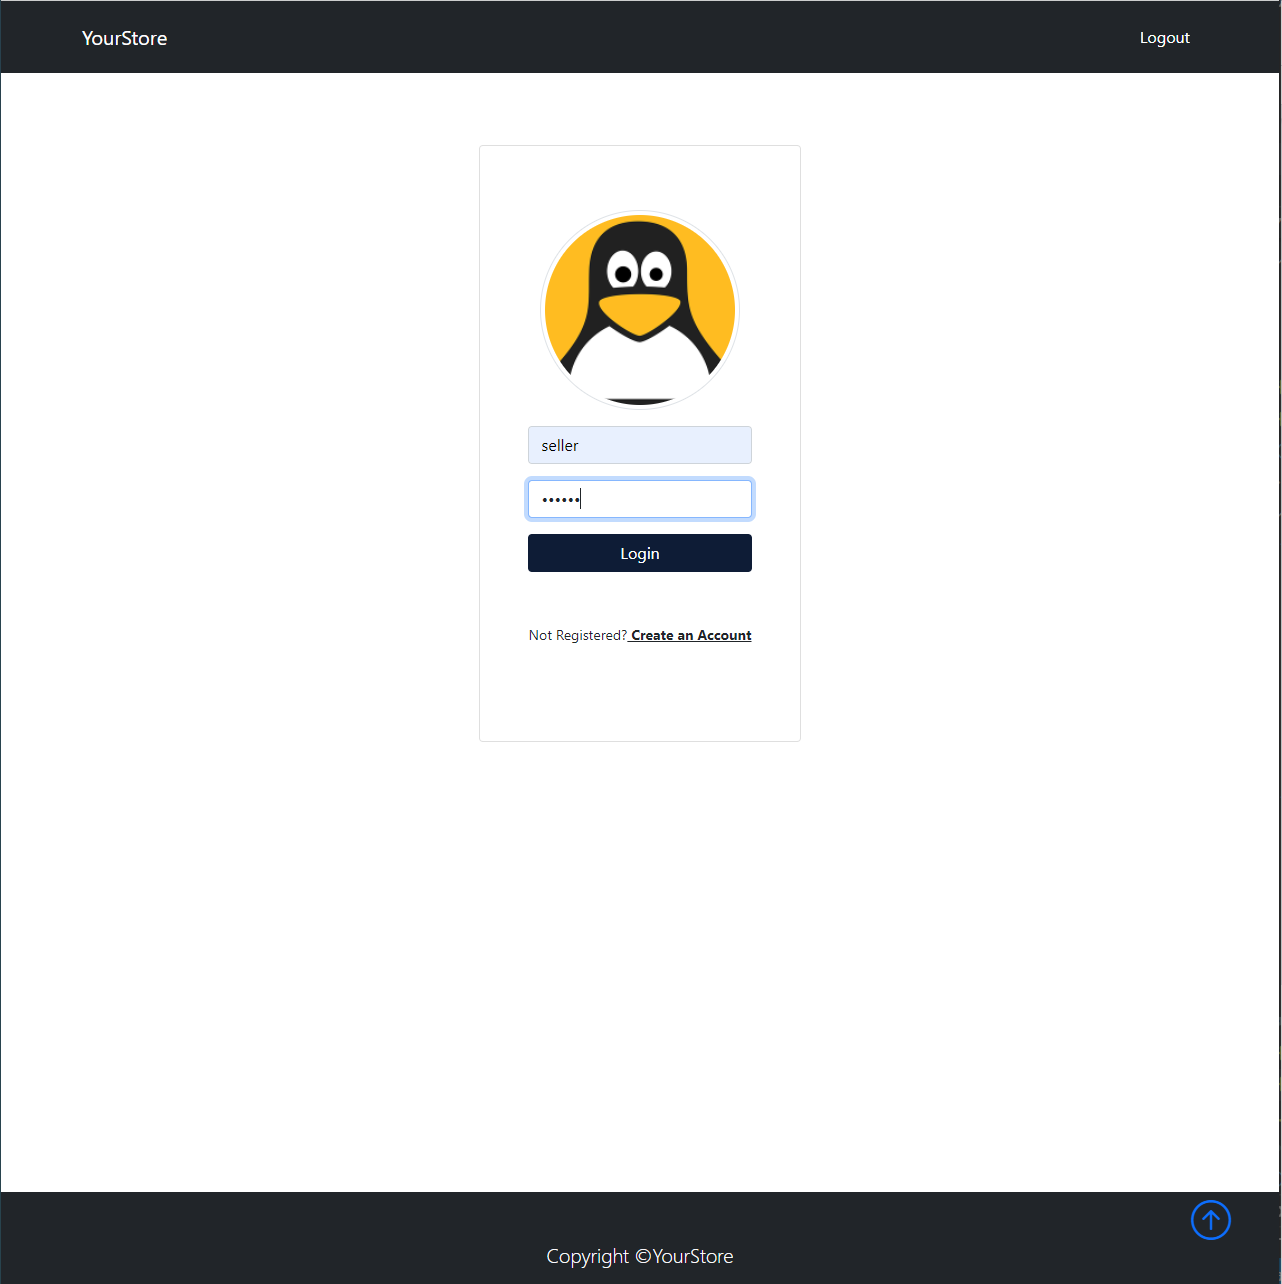
\includegraphics[width=0.45\textwidth]{UserGuideImage/7.png}


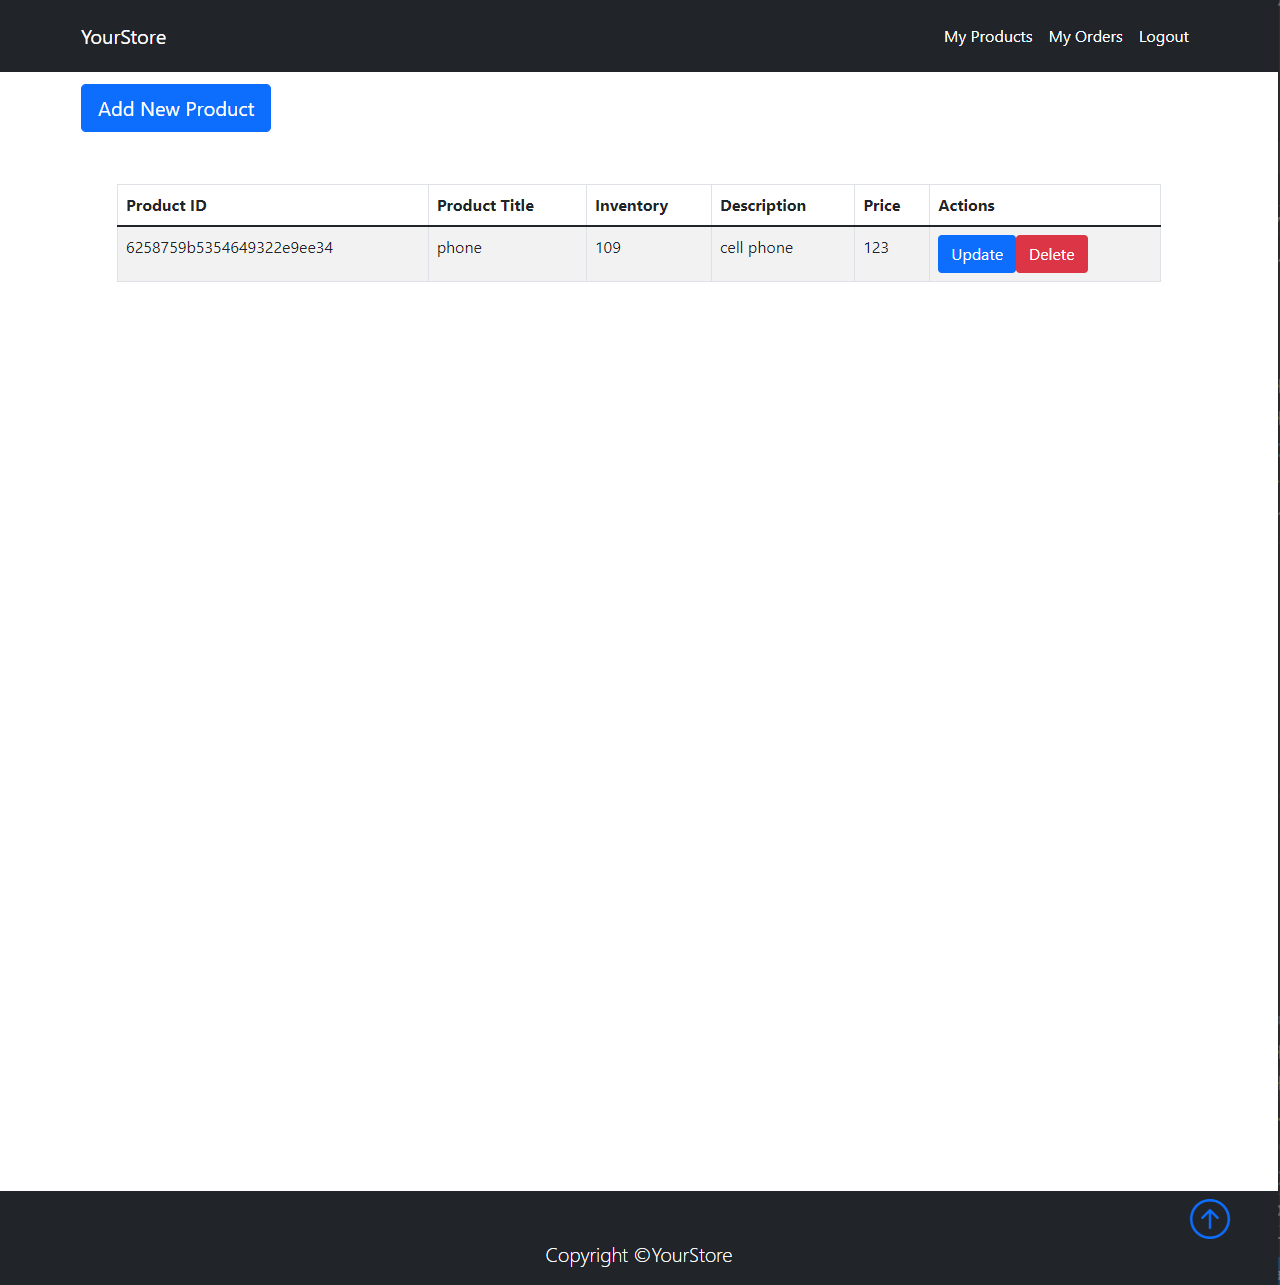
\includegraphics[width=0.45\textwidth]{UserGuideImage/8.png}

\newpage
\textbf{5: Seller manage products}

You can access “My Products” page by automatically sign in as seller or click “My Products”
at nav bar. In “My Products” page, seller can create a new product as below by clicking "Add New Product".

\vspace*{5mm}
\hspace*{5mm}\textbf{5.1: Create a new product}

Filled in all the blanked fields, and click "Create Product" to actually create the product.

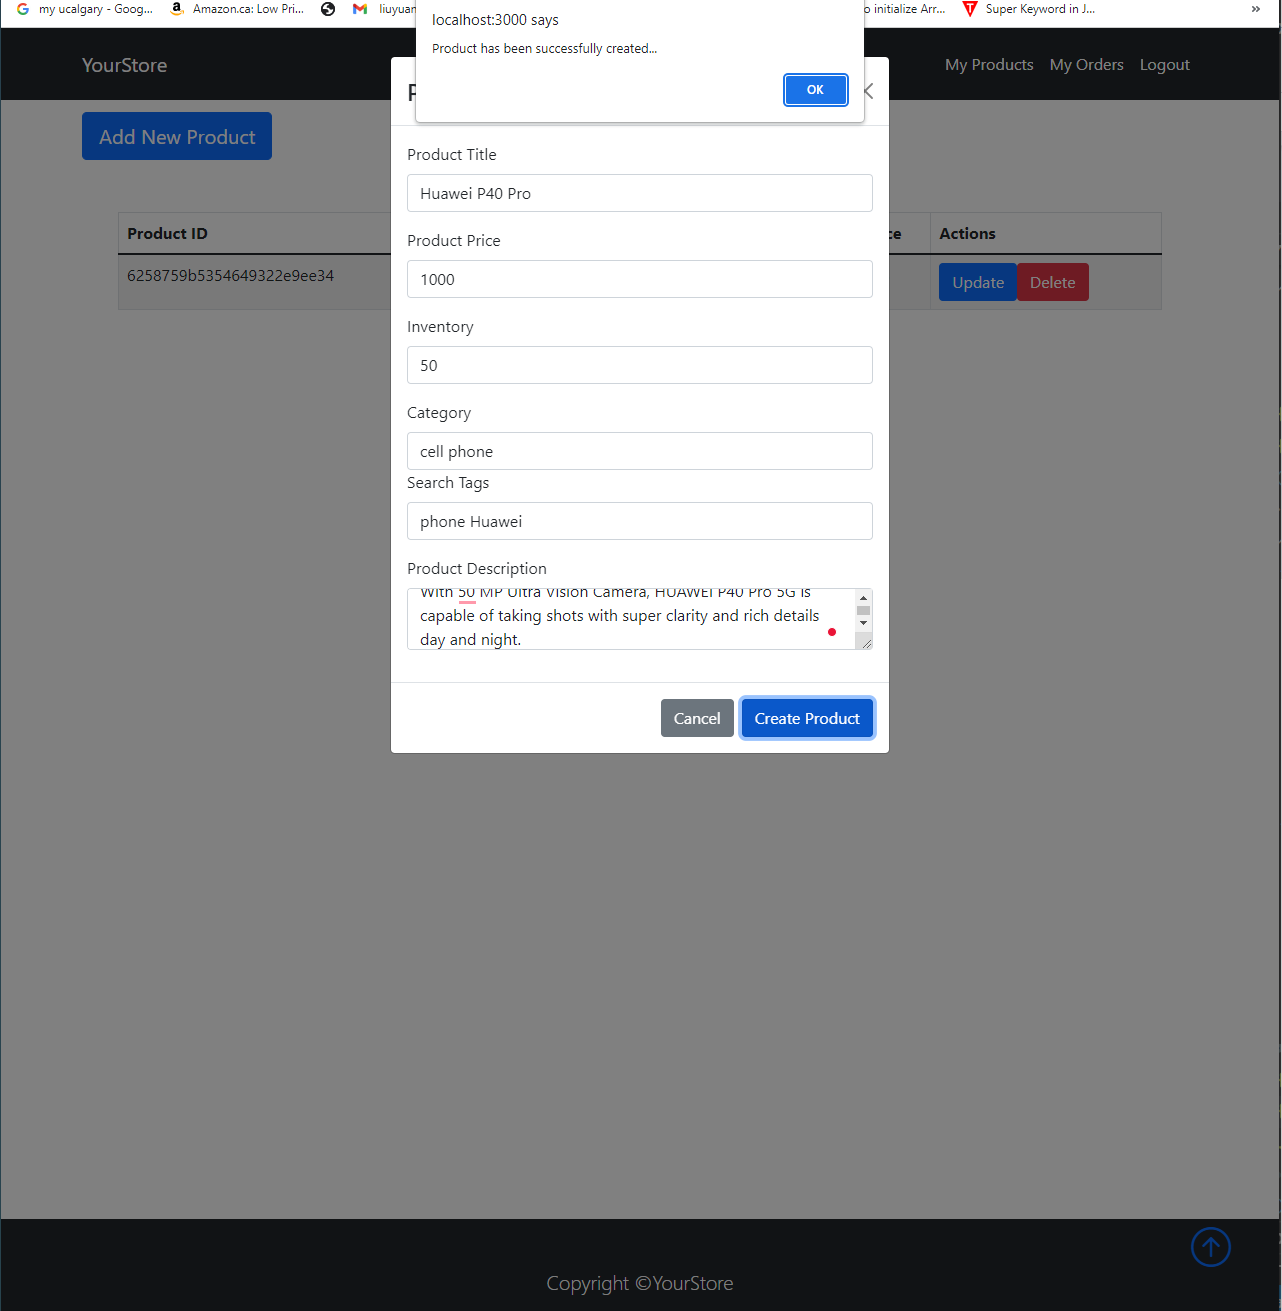
\includegraphics[width=0.45\textwidth]{UserGuideImage/9.png}

\vspace*{5mm}
\hspace*{5mm}\textbf{5.2: Update/Delete products}

You can choose to update or delete product by click corresponding buttons.

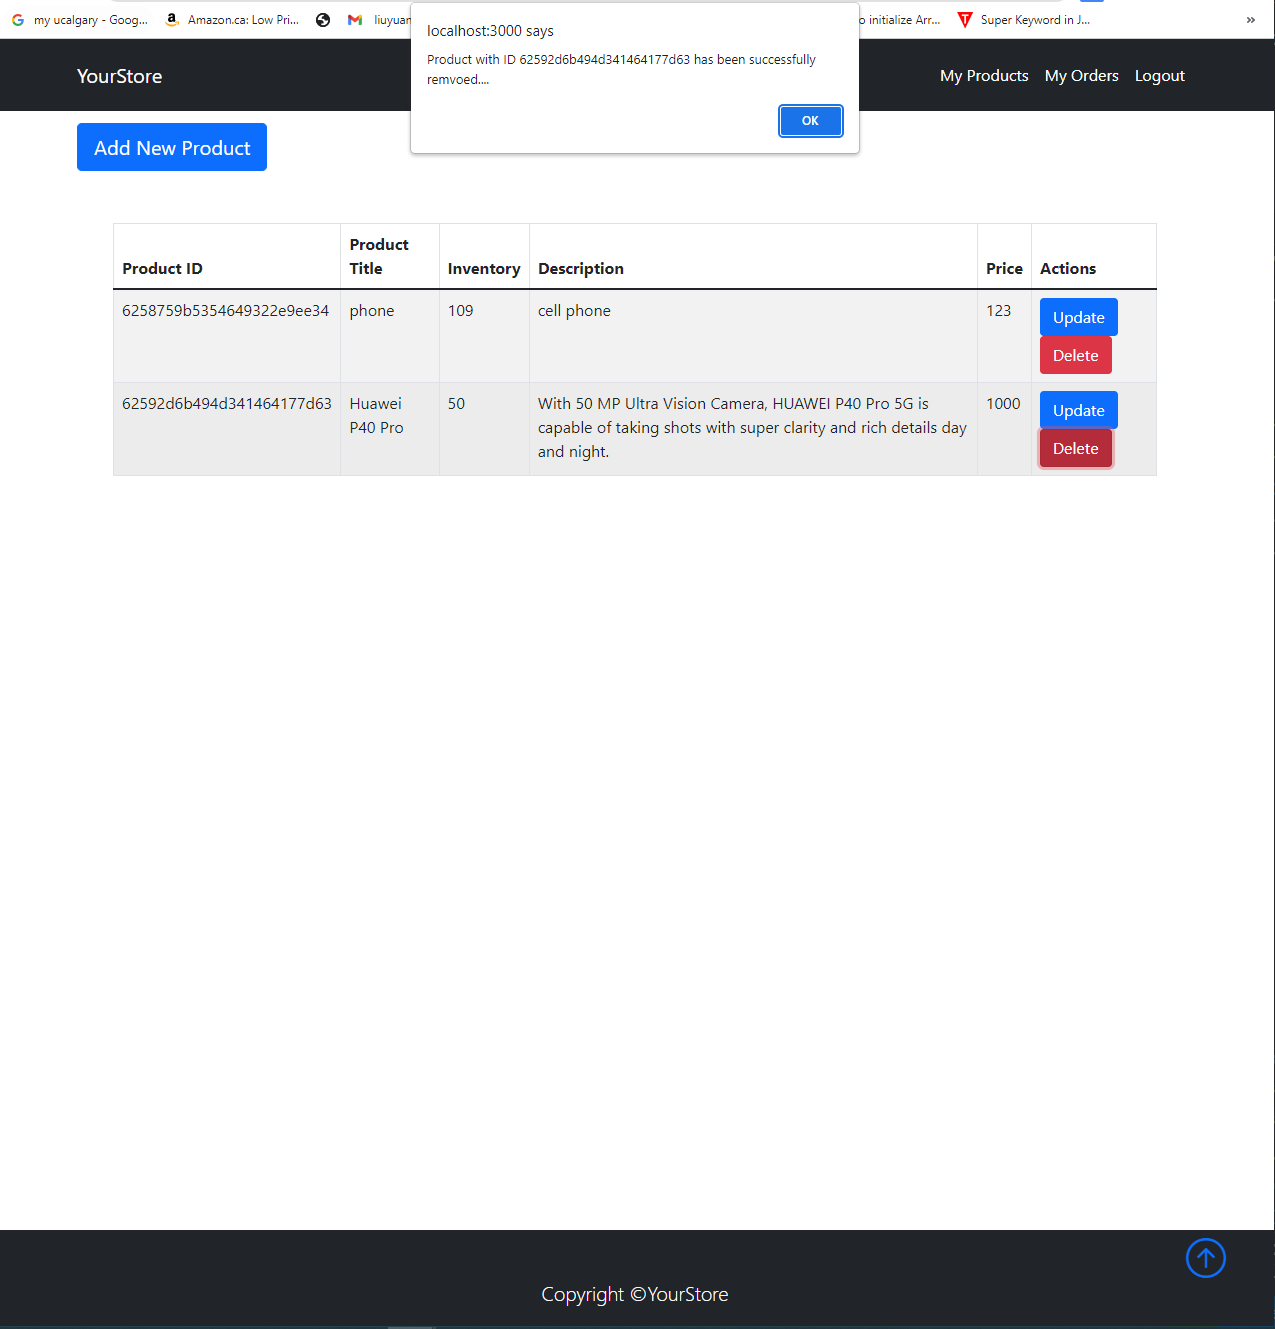
\includegraphics[width=0.45\textwidth]{UserGuideImage/10.png}

\newpage
\textbf{6: Seller manage orders}

Click “My Orders” on nav bar, seller can update/delete any existing orders as below.
Note that you only need to fill in the fields that need to be updated.

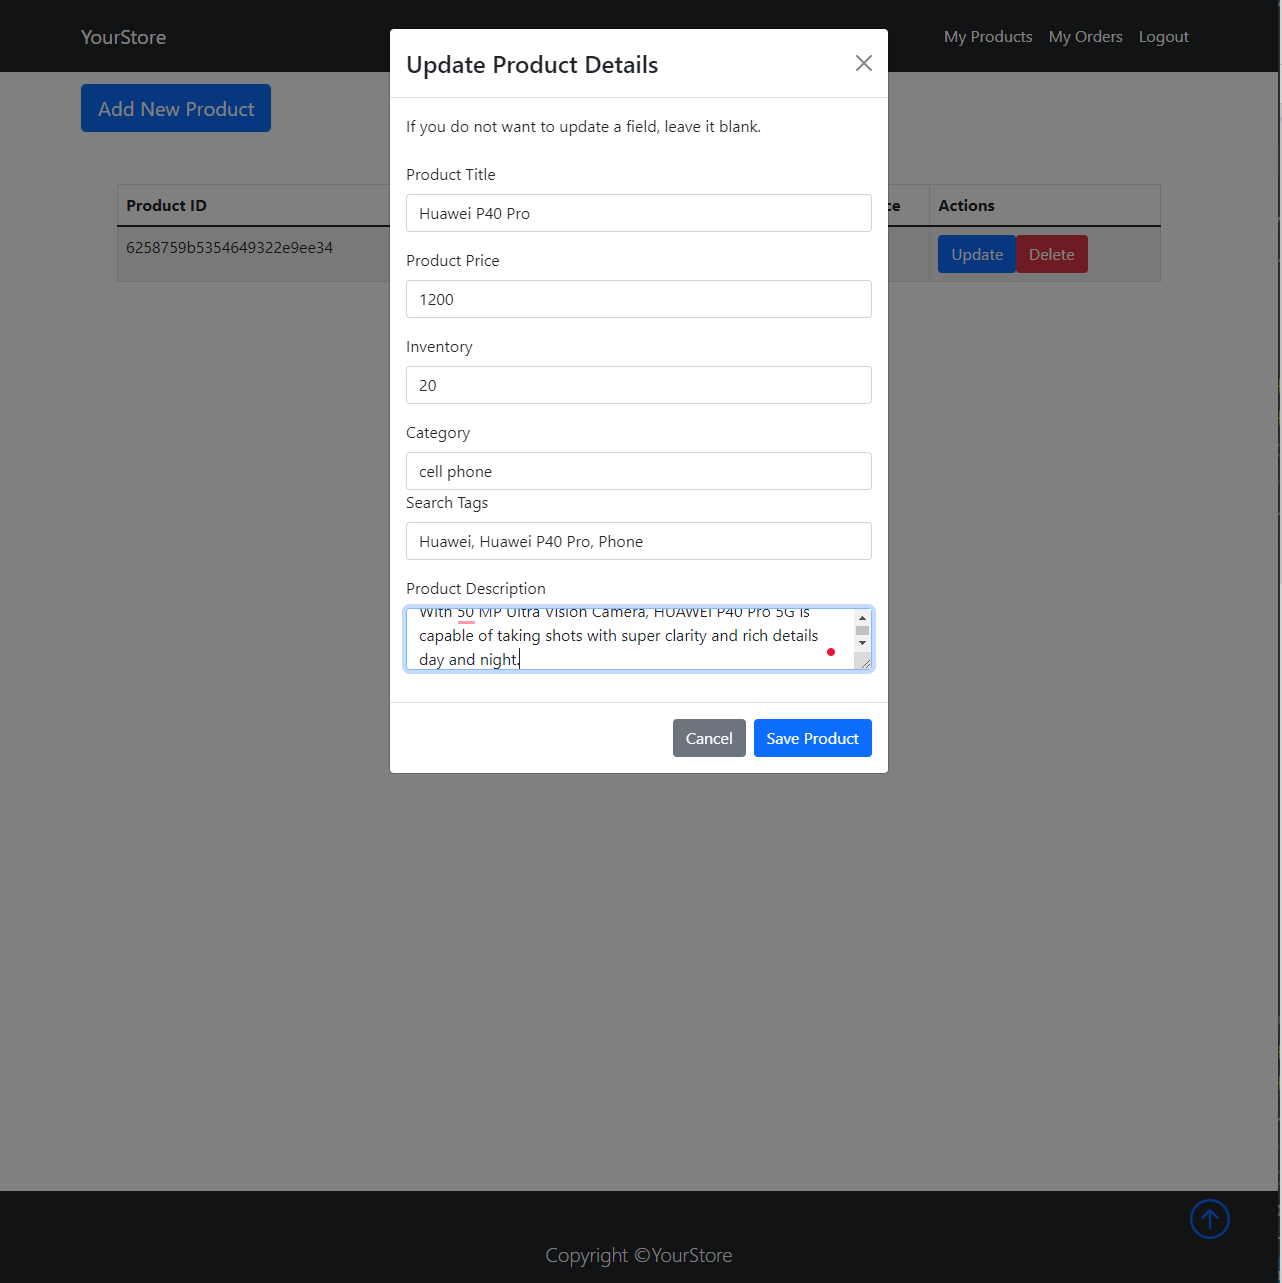
\includegraphics[width=0.45\textwidth]{UserGuideImage/11.png}


\newpage
\textbf{7: Sign in as customer}

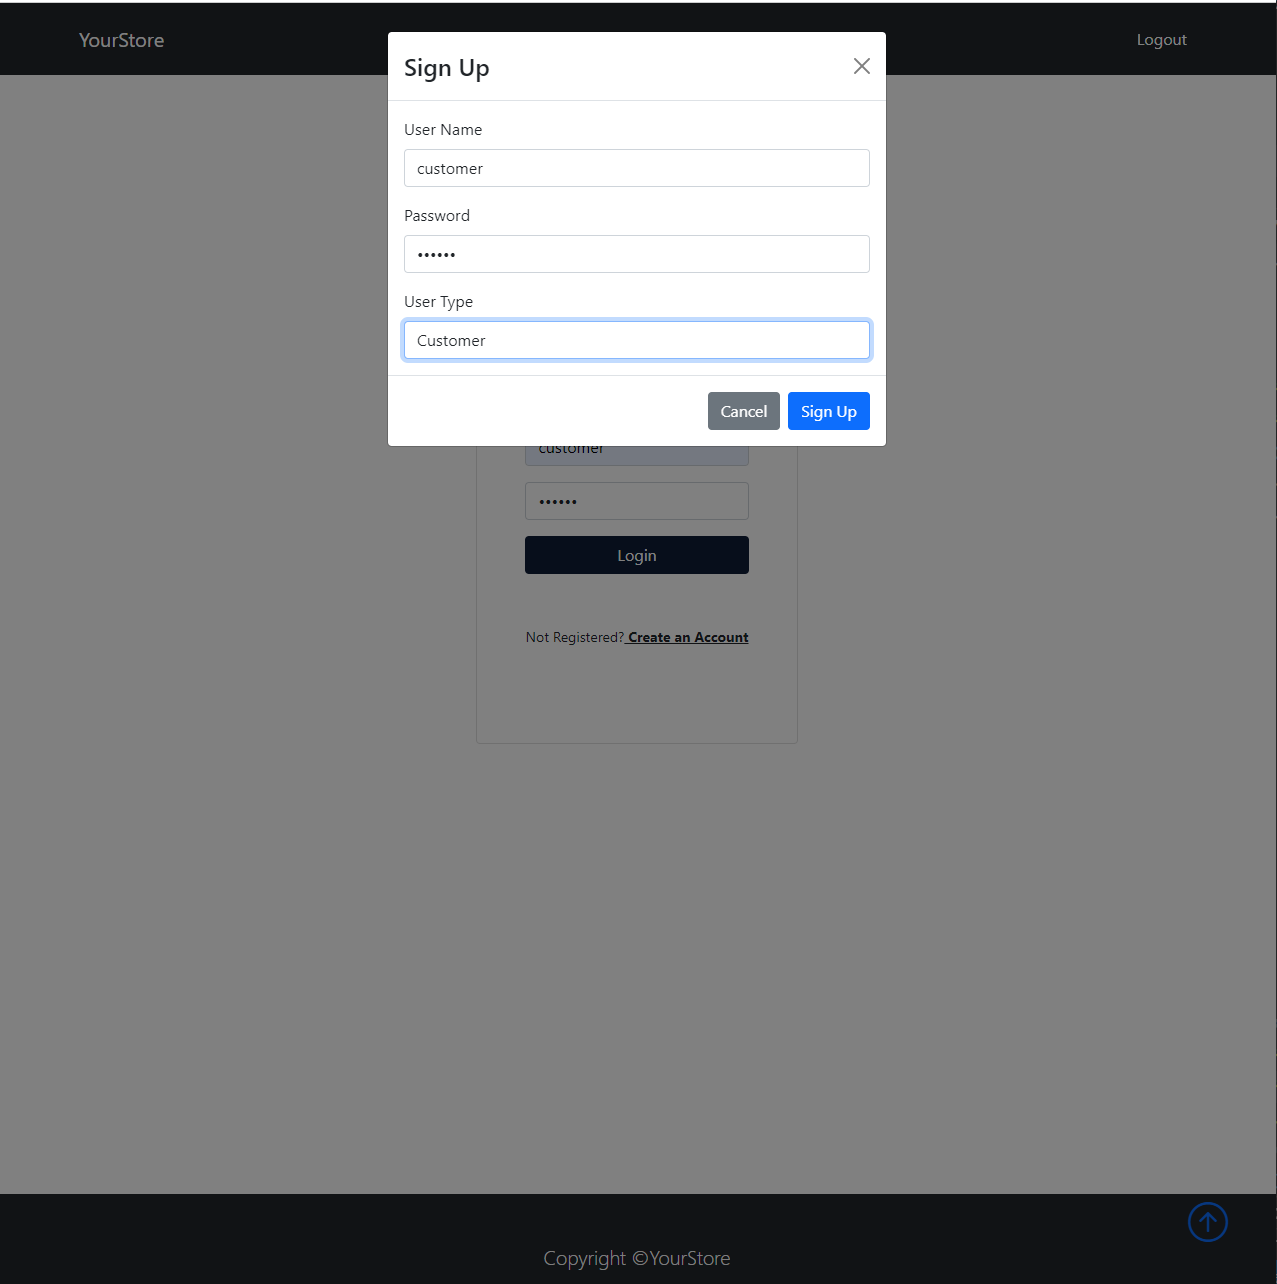
\includegraphics[width=0.45\textwidth]{UserGuideImage/12.png}
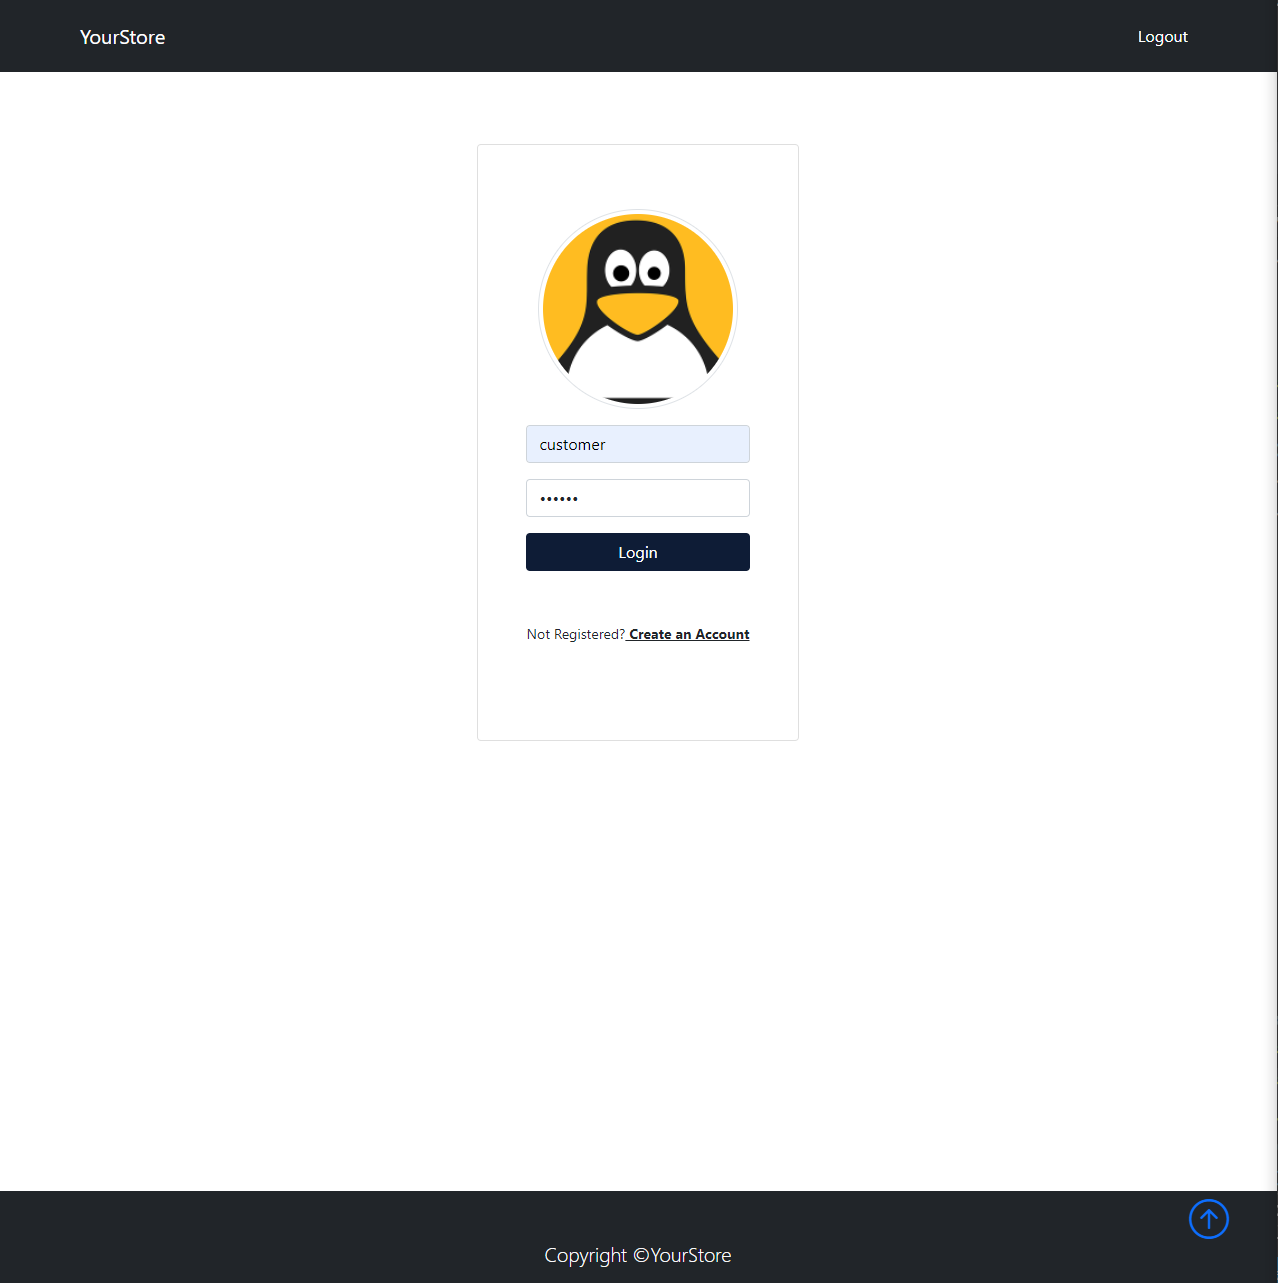
\includegraphics[width=0.45\textwidth]{UserGuideImage/13.png}

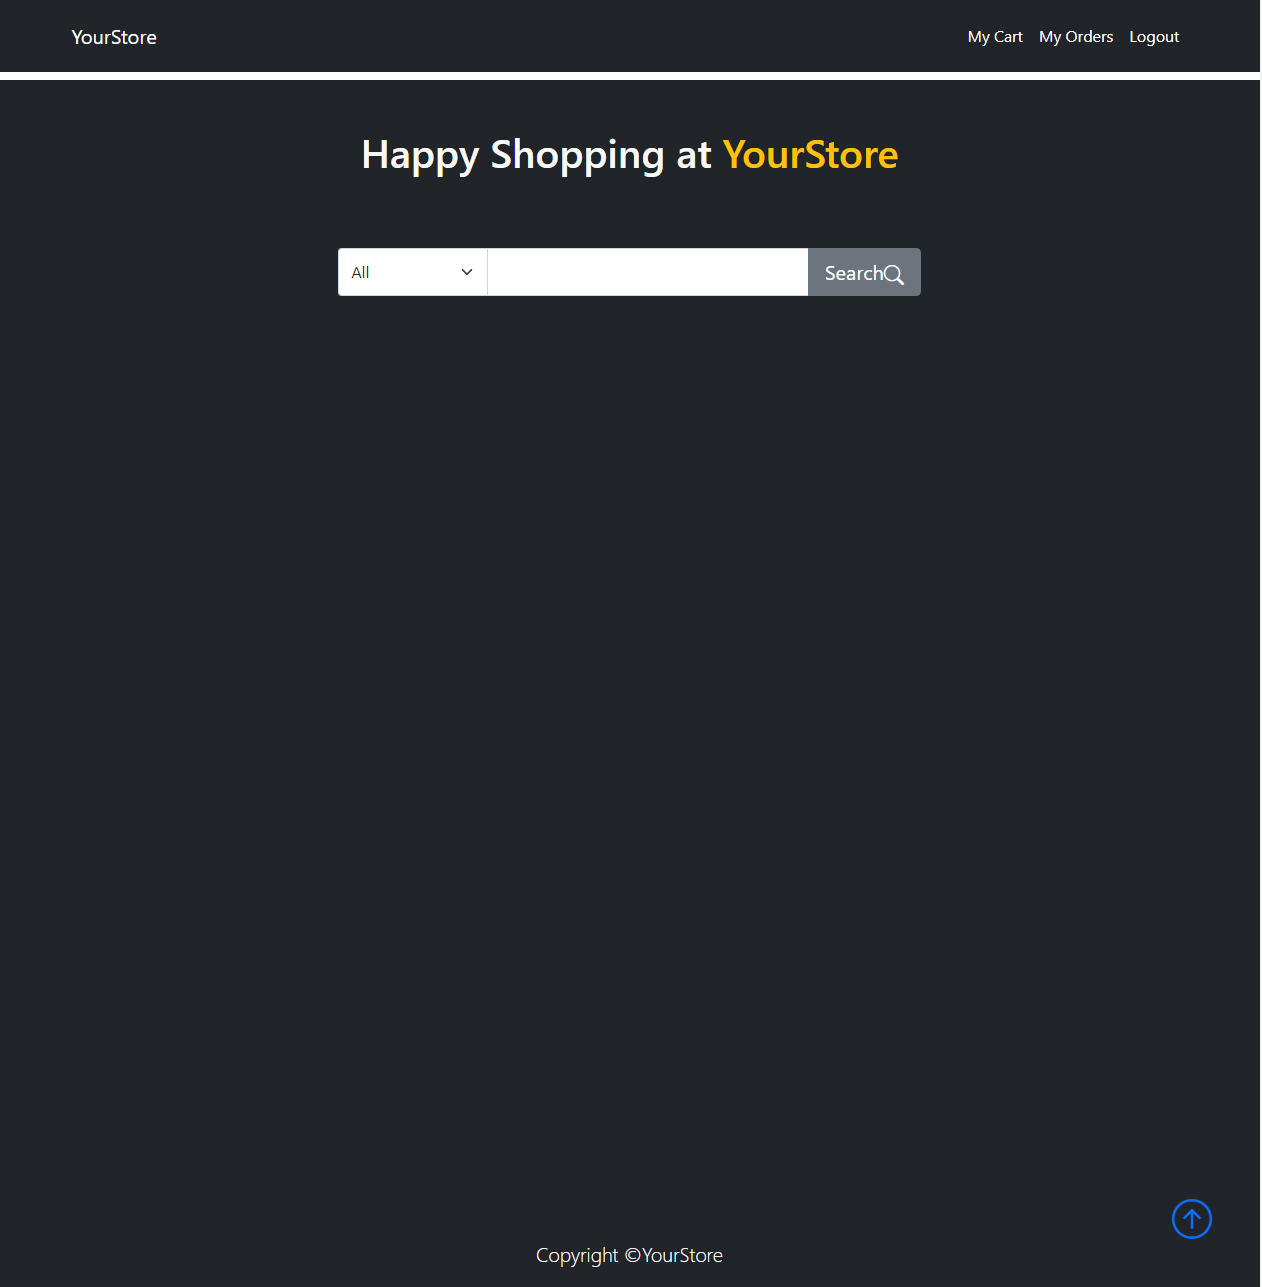
\includegraphics[width=0.45\textwidth]{UserGuideImage/14.png}

\newpage
\textbf{8: Customer add product to cart}

After searching the products, the customer can choose his/her favorite product and click "Add To Cart" button
to add the product into the cart.

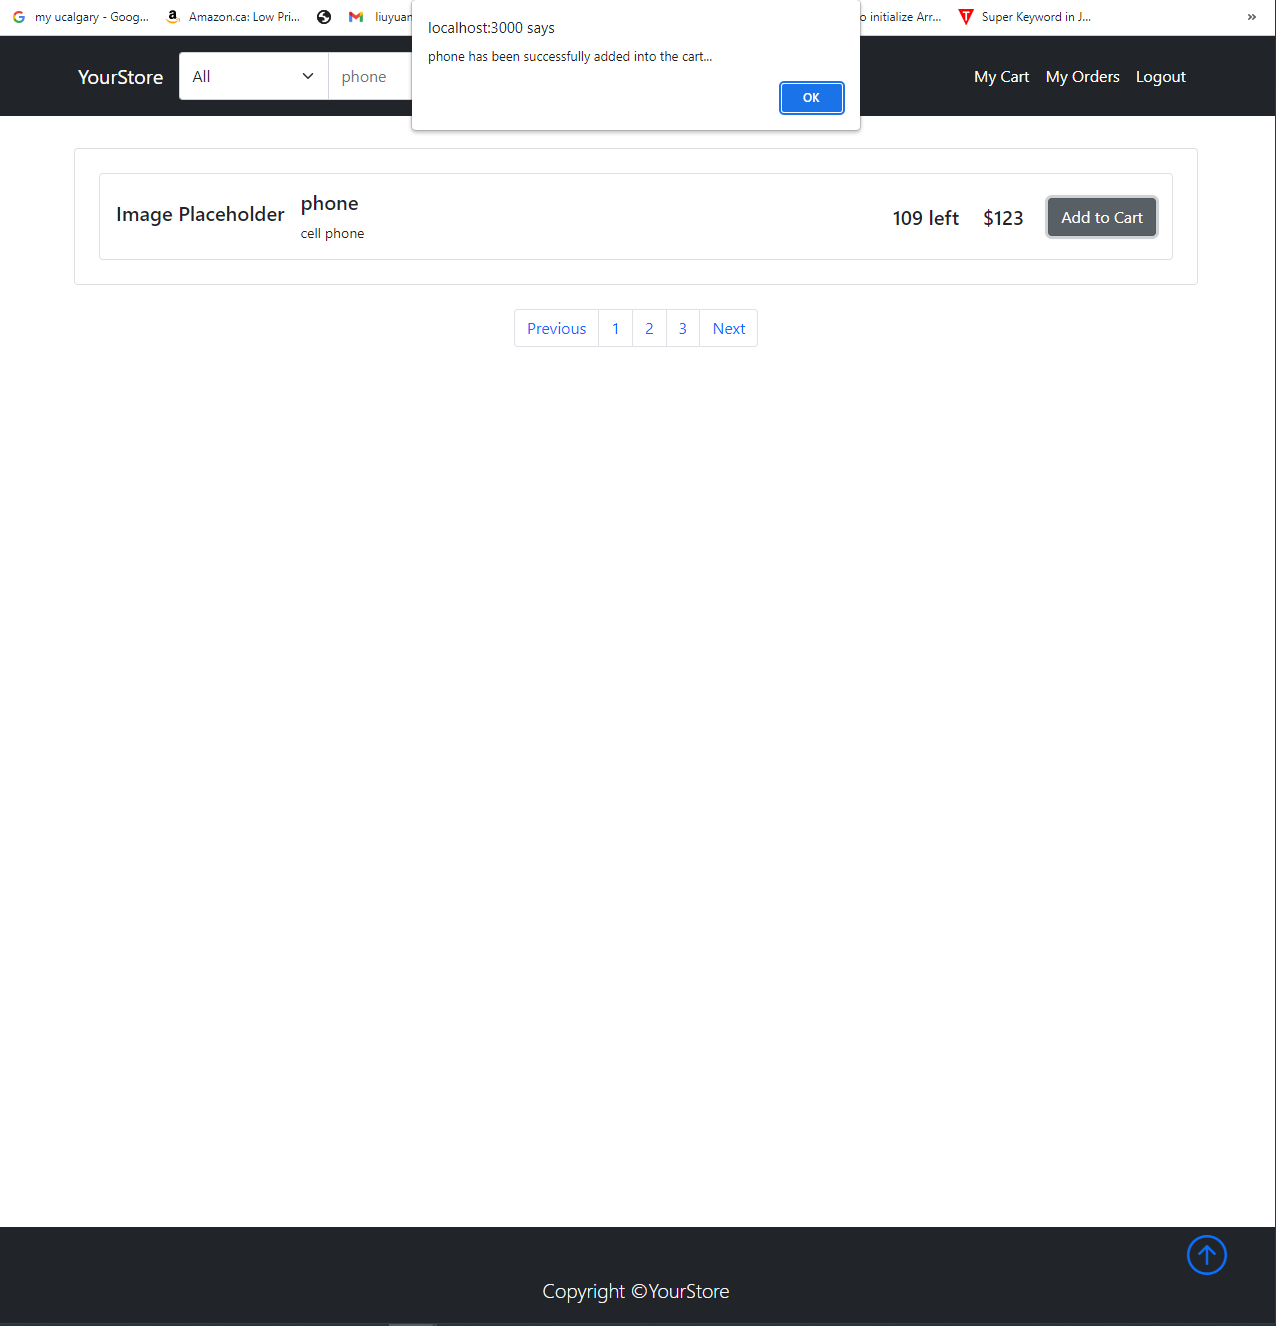
\includegraphics[width=0.45\textwidth]{UserGuideImage/15.png}

\vspace*{5mm}
\textbf{9: Customer place order}

The customer can navigate to his/her cart by clicking "My Cart" on the navigation bar. After examing
the cart carefully, the customer can fill in the receiver details in the grey box and click "Purchase" to create orders.

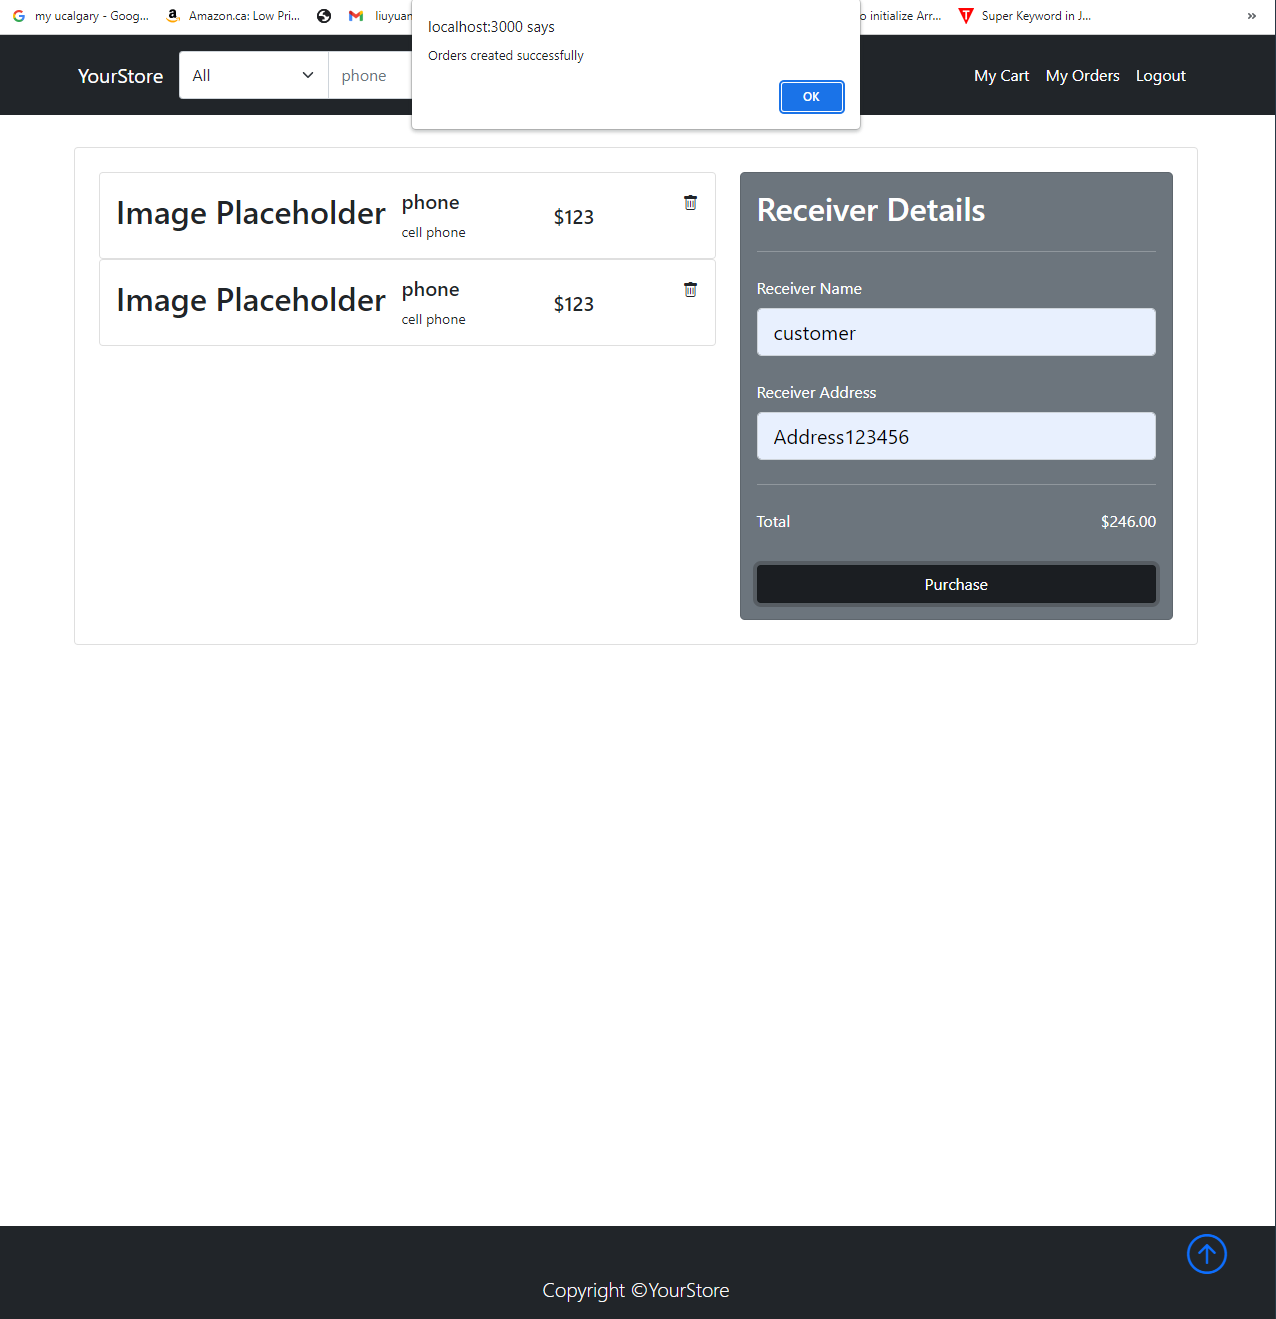
\includegraphics[width=0.45\textwidth]{UserGuideImage/16.png}

\newpage
\textbf{10: Customer manage order}

After click "My Orders" link in the navigation bar, the customer should be redirected to a page that he/she can manage
his/her orders. The customer can choose to "Pay" for the order or "Cancel" the order by clicking
the corresponding buttons.

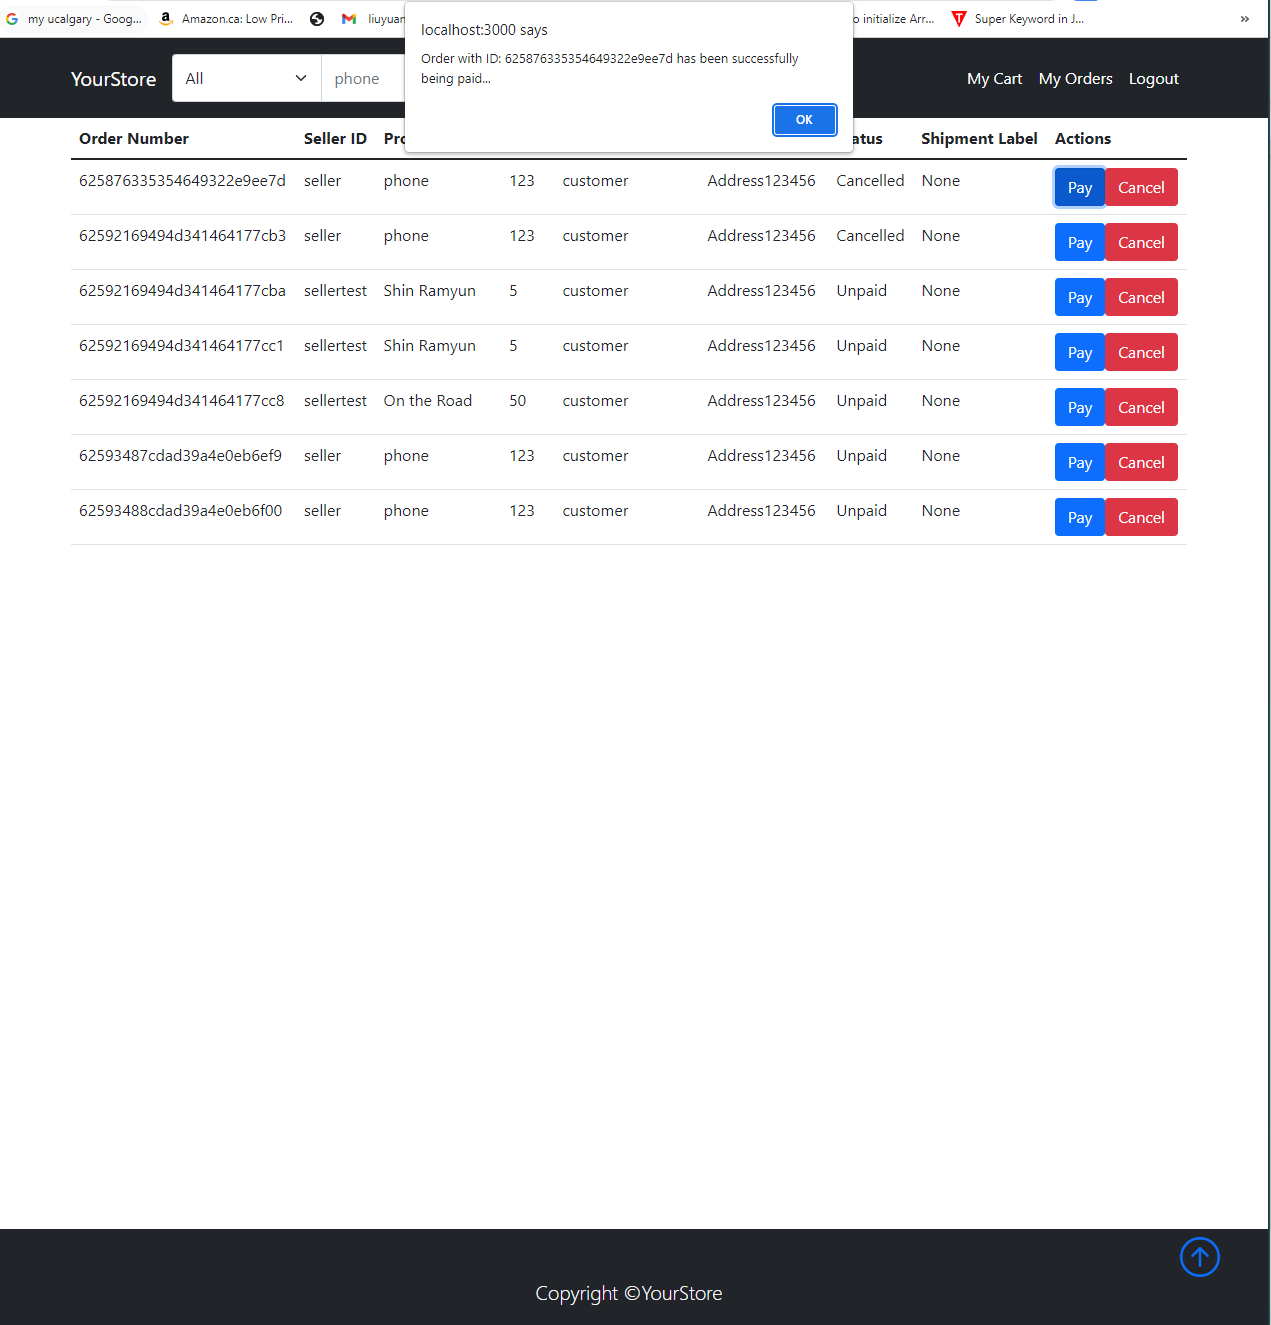
\includegraphics[width=0.45\textwidth]{UserGuideImage/17.png}


\end{document}